\chapter{Theory}
\label{chap:theandme}
This chapter is divided into three parts. The first part introduces basic concepts of linguistics and natural language processing. With the focus of this work in mind, deep learning basics are presented in the second part. The third part of this chapter offers a more detailed explanation of methods directly relevant to this work (especially the BERT model).

\section{Linguistics and \acrlong{nlp}}
\acrfull{nlp} can be described as a science at the border of linguistics and computer science. However, according to \citep{Wilks}, \acrshort{nlp} itself is not a scientific research subject. It is instead a collection of problems, which can be examined. These tasks are taken from the general linguistics field, and the goal is to solve (or \textit{process}) them by computers. The study subject of linguistics is language and its description. The focus of linguistics can be divided into the following sub-fields: phonetics, phonology, morphology, syntax, semantics, and pragmatics. This work focuses on morphology (lemmatization, \acrfull{pos} tagging) and semantics (sentiment analysis) tasks. A more detailed description of tasks can be found in the following subsections and dedicated chapters for each task. Apart from the introduction of tasks, this chapter also includes a brief \acrshort{nlp} history overview and a presentation of possible data sources for \acrshort{nlp} training.

\subsection{Morphology}
Morphology studies an internal structure of words. Morphological tasks can be divided into generative and analytical. Generative tasks for a given word focus on the generation of word form for a given grammatical category. On the contrary, analytical tasks try to find  e.g. a part of speech tag or a grammatical categories of the given word. Both of these types of tasks are important for \acrshort{nlp}. 
\par
This work performs two morphological analytical tasks - lemmatization and \acrfull{pos} tagging.
%The result of morphological analysis is a set of possible lemmas and tags (described bellow) for a given word form. This set can be further narrowed by lemmatization (selection of the one "right" lemma), morphological tagging (selection of one correct tag in the given context), or partitional disambiguation (removes all tags and lemmas, which can be reliably removed). 
%These forms can be useful for machine translation, full-text searching, labeling documents by their keywords, or spell-check.

\par
\subsubsection{Lemmatization task}
Lemmatization task consist of finding a \textit{lemma}. Lemma is one chosen form of a word, selected to represent the whole set of all possible word's forms (such set is called lexeme).  A convention chooses word form used as lemma -- it is nominative of singular for a noun, an infinitive for a verb, etc.
\par
For example, lexeme for a Czech word \textit{jablko} is \textit{jablko, jablka, jablku,  jablkem, jablek, jablky, jablkům} and the lemma is \textit{jablko}.

\subsubsection{\acrshort{pos} tagging} 
\acrshort{pos} tagging classifies word into one of the \acrshort{pos} categories (like a noun, pronoun, or verb) \citep{Hladka}. As a part of tagging task can sometimes be considered a determination of grammatical categories (e.g., case, number, or tense). 

\subsection{Semantics}
Semantics deals with word meaning. This is a more challenging study than morphology, even for humans, let alone for computers. The most important reasons are that word meaning can be subjective, change during historical periods, a sentence is not a simple sum of meanings of its words and moreover it is not clear how to represent meaning in the computers.
\par
Semantic analysis can be useful for various tasks, from natural language text generation to recognizing homonymy\footnote{Homonyms are words, which share same spelling or pronunciation, but they have different meaning.} or polysemy\footnote{Polyseme is a word with many different, but related meanings.} of given words. It could solve sophisticated assignments as answering questions about the input text document or help in high-quality translation, finding so-called named entities (like persons, months, or cites) ,linking these entities to some knowledge base, or analysing sentiment (which is one of tasks solved in this thesis).

\subsubsection{Sentiment analysis}
An input of sentiment analysis is a text, and the output is a classification into one of the categories. In this work, categories are positive, negative, and in some datasets also neutral, but it is common to use labels like abusive or ironic, too.
As a part of sentiment analysis can be involved so-called subjectivity\citep{Montoyo2012}. The subjectivity prediction goal is to classify if the
opinion (both positive or negative) is objective or the author is personally interested and has strong emotions about his claims. For example, the following text could be recognized as objective: "The sound of this notebook is clear.", "The base is not stable enough." or even "An internet connection in this area is bad." in contrast with "I hate the way the new touchpad works.", which is highly subjective. The subjectivity of the claim does not depend on its sentiment. This work treat only positive/neutral/negative classification, not a subjectivity analysis.

\subsection{Language data}
Data of many kinds can serve as an input into natural language processing, and this data can be categorized by a form or by source.
As for form, we can work with corpora or datasets of various sizes, containing data from many sources. A corpus is a large collection of texts, aiming to be a representative sample of a language. This is not entirely possible, mainly because the selection of examples in the corpus is limited compared to language diversity. Despite these limitations, corpora are a valuable source of language information and are widely used in \acrshort{nlp}. The most famous linguistic corpora are co-called Brown corpus \citep{francis79browncorpus} -- first electronic corpus mixed from newspaper articles and fiction literature, and PennTreebank \citep{Marcus1993}, which is the first syntactically annotated corpus but has quite a domain limited source - articles from Wall Street Journal. Corporas can differ in an internal structure. One of corpora's type is a treebank. A treebank is a corpus with many possible types of annotations that uses trees to represent dependencies. An example of such trees can be seen in figure \ref{fig:trees} and an example of a treebank is presented in picture \ref{fig:pdt}.
The question arises as to what is the difference between a corpus and a "simple" dataset. Sometimes these terms can be interchangeable in the sense that the usage of both can be the same. Both types of data can be used for the same task, but the difference can be seen in a purpose of a collection. A corpus's idea is to collect a somehow representative sample of a language with annotations on many levels, which allows the performance of various analysis upon this data. Dataset is typically created on a restricted domain and they are annotated for one type of task, e.g. tweets on US Airlines pages \footnote{https://www.kaggle.com/crowdflower/twitter-airline-sentiment} or movie reviews \footnote{https://www.kaggle.com/lakshmi25npathi/imdb-dataset-of-50k-movie-reviews}, which are an example of such sentiment analysis datasets.
\begin{figure}[ht]
\centering
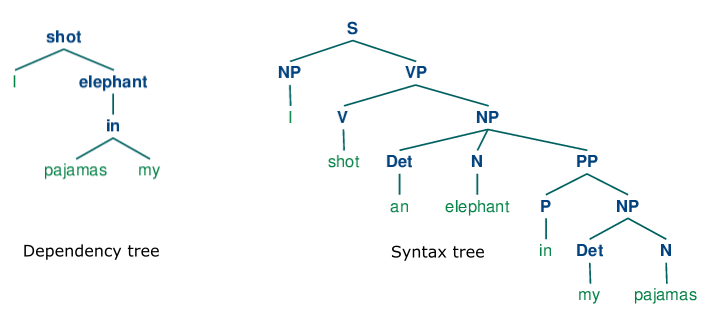
\includegraphics[width=1\textwidth]{../img/syntax_depedency_trees.png}
\protect\caption[LoF entry]{
An example of the syntax and dependency tree. The dependency tree, as the name indicates, describes dependencies between words. Such dependencies are of various types; for example, an elephant in the example text is a direct object of the shooting action. \par A root of such a tree is typically a predicate of the sentence. On the other hand, the syntax tree represents the sentence's syntactic structure according to the grammar. The root of the tree is \textit{sentence}, which is split into noun and verb phrase. These can be further divided into phrases compound from particular instances of parts of speech (e.g., nouns, adverbs, verbs, prepositions, etc.).
\newline \textit{Source: \cite{NLTKbook}}
}
\label{fig:trees}
\end{figure}

\begin{figure}
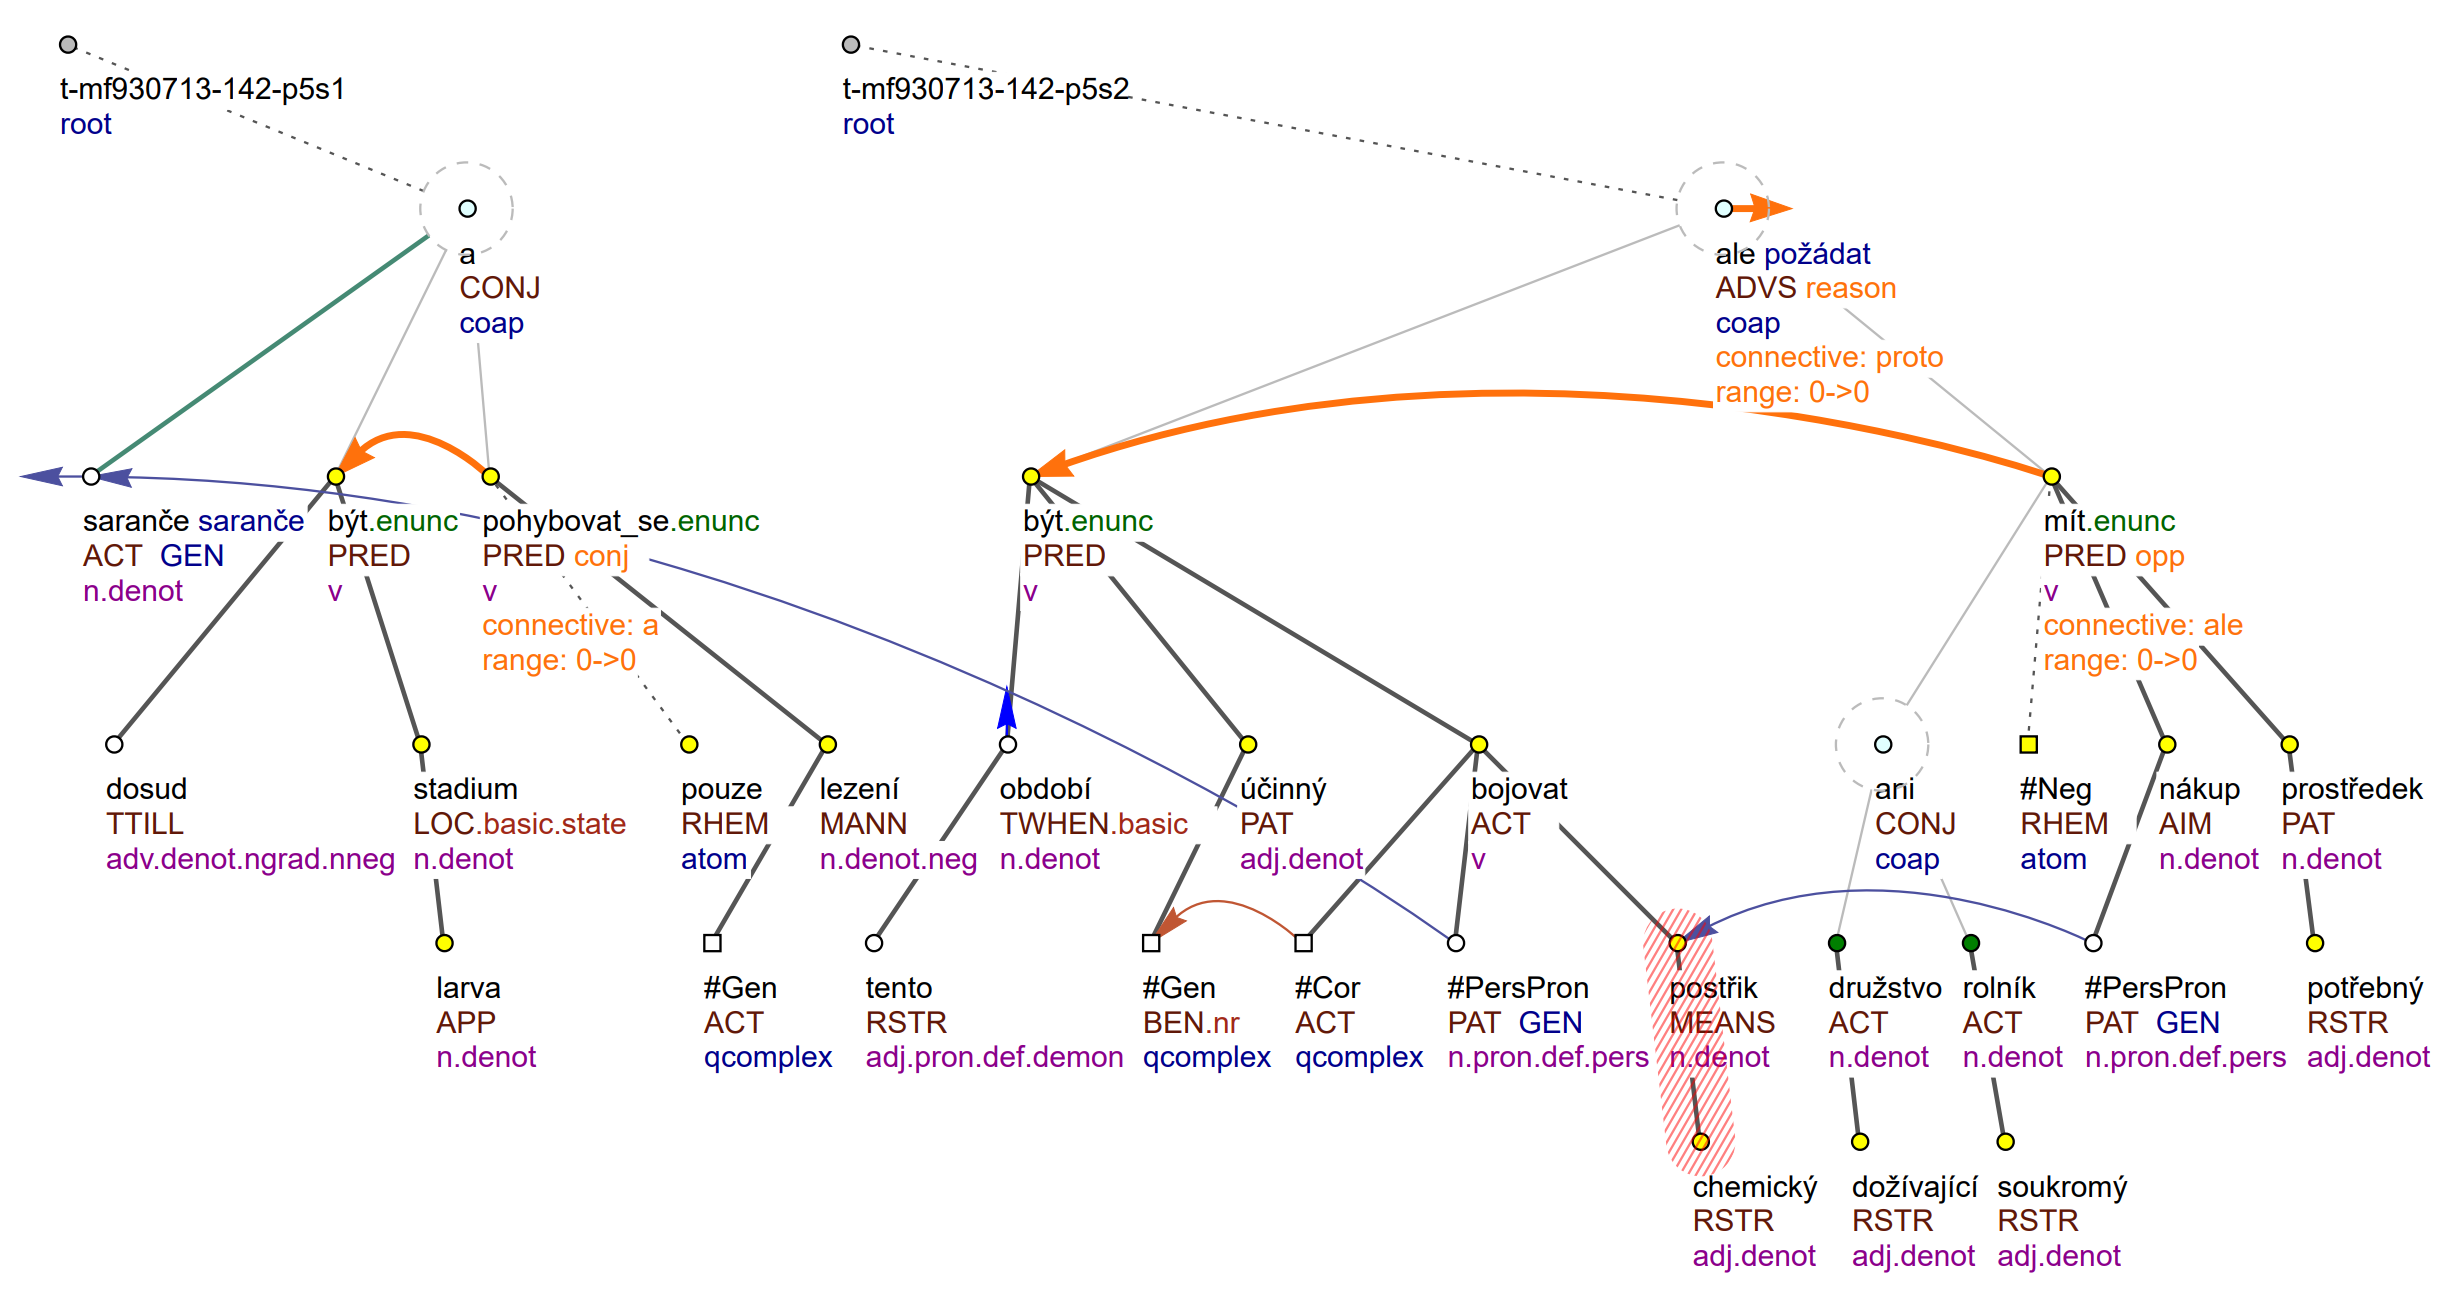
\includegraphics[width=1\textwidth]{../img/prague_dep_treebank.png}
\caption{
Prague dependency treebank example \cite{PDT35} for the sentences:
\textit{Grasshoppers are still in the larvae stadium, crawling only. At this time of the year, it is efficient to fight them using chemicals, but neither the ailing cooperatives nor private farmers can afford them.} czech: \textit{Sarančata jsou doposud ve stadiu larev a pohybují se pouze lezením. V tomto období je účinné bojovat proti nim chemickými postřiky, ale dožívající družstva ani soukromí rolníci nemají na jejich nákup potřebné prostředky}. This treebank contains dependency trees, but is is just one of many possibilities. Prague dependency treebank offers different layers of annotations. Red strips over words \textit{chemický} and \textit{postřik} marks multiword phrase, conjunction between \textit{rolník} and \textit{družstvo} is expressed as by one type of nodes, blue lines denotes coreference etc.} Praque dependency treebank data are used for tagging and lemmatization tasks.
\label{fig:pdt}
\end{figure}

Data in both dataset and corpora can come from many written or oral sources. For example, in machine translation task, documents with many language versions are appropriate. An example of the use of such multilingual documents was a project Eurotra \citep{oakley1995final}. Linguistic data can, however,  differ in quality and length.  A relatively new source of data are social networks like Twitter, Reddit, or Facebook. Data from some social networks (Facebook, Twitter) are very different from traditional sources like scientific papers, newspaper articles, or books.  These data are short snippets of text full of odd characters, newlines, and ends of lines. They contain pictures, emojis, a mixture of different languages, slang expressions, and grammatical errors. Furthermore, they are very short; sometimes, they consist only of one sentence, few hashtags, and a link or a picture. Because people share their opinions and emotions and are ready to make their choices according to incoming influences, social networks are for some areas one of the most important source of information. The big problem while analyzing this data is their amount. Twitter users, for example, produce about 12 TB of data per day \footnote{https://bigdatashowcase.com/how-much-big-data-companies-make-on-internet/}. It is impossible to process all the data manually, so this is one reason for the rising industry importance of natural language processing.

\subsection{Historical Development}
The historical development of computer linguistics was significantly affected by machine translation \citep{Wilks}. \acrshort{nlp} was improved by some of the milestones in machine translation history, therefore its historical development will be presented as well. First machine translation attempts formally started in 1933 by patents for machine translations (mechanical multilingual dictionaries) \citep{Hutchins}
followed by a big boom of machine translation in the 50s and 60s and then continued by a slowdown after ALPAC report in 1966 \citep{Hutchins1996}. 

The first solutions to machine translation tasks were based on bilingual dictionaries and sets of rules. This method translated an individual word or a small group of words with a subsequent improvement of syntax and morphology. The resulting translation was not good and required lots of human work of expert linguists. This approach was replaced around the year 1990 by a statistical translation \citep{Brown}. A statistical machine translation's central idea is a probability of a translated sentence, given the original sentence. This includes also a probability of resulting sentence in the target language. This probability distribution is called a language model, and although it is one of the most aged ideas in \acrshort{nlp}, it is an integral part of current best \acrshort{nlp} solutions. Words probabilities were originally computed using frequencies of words or sequences of n rows (so called n-grams) in large language corpus \citep{jurafsky2012natural} (for more information about probabilistic language models, see subsection \ref{sub:models}). These methods were quite successful, but they suffered from the curse of dimensionality \footnote{Curse of dimensionality is a problem connected to the data with many variables. In such high-dimensional space, distances between samples are so big that it makes really difficult to distinguish between similar and completely different samples or find some meaningful pattern in the data.} \citep[p.450]{Goodfellow-et-al-2016}. The next stage of machine translation (and other \acrshort{nlp} tasks) starts with the second wave of neural networks' popularity \citep{Goldberg},\citep{Google}. There are too many possible words or n-grams of words, and there is no way to share learned information between similar words or sequences in statistical methods. A solution to this problem is an invention of word embeddings \citep{Bengio2003} (see \ref{sec:embedd}). Neural language models (a neural network which learns probabilities of words) obtained even better results \citep{Schwenk2006}. Current natural language processing is built on deep recurrent neural networks and encoder-decoder architecture, firstly published in \citep{Cho2014}, \citep{Sutskever2014} and \citep{Wu2016}. 
\section{Deep Learning}
In current times, neural networks are applied to machine translation and almost any other linguistic tasks. State-of-the-art result for machine translation, sentiment analysis, and many others is held by methods based on deep learning \footnote{http://\acrshort{nlp}progress.com/}. Also the main focus of this work is on neural entowrk methods. For that reason, this section presents deep learning basics, their usage, and improvements in \acrshort{nlp} in recent years. 

\subsection{Deep Learning History}
The history of learning algorithms inspired by a human brain started in the 1940s under the name \textit{cybernetics} \citep{Goodfellow-et-al-2016}, \citep{McCulloch}. The first such architecture was a perceptron \citep{Rosenblatt1958}.
Perceptron, invented in 1958, is the most straightforward neural network with just one layer serving for binary classification (see Fig. \ref{pic:perceptron}). A perceptron's input is a vector of features describing an input example, and output is a classification into class 0 or 1.

\begin{figure}[ht]
\centering
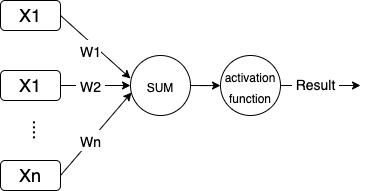
\includegraphics[width=0.8\columnwidth]{../img/perceptron}
\caption{A one-layer perceptron architecture. The result is formed by the application of the activation function on a weighted sum of inputs. Weights are updated during training till it returns satisfactory results. }
\label{pic:perceptron}
\end{figure}

There also exists a multi-class version for the general classification,  but perceptron also had limitations. The problem of the perceptron was the inability to classify data that are not linearly separable \citep{Minsky2017} (see Fig. \ref{pic:xor}), which led to a lack of interest in deep networks for some period.

\begin{figure}[ht]
\centering
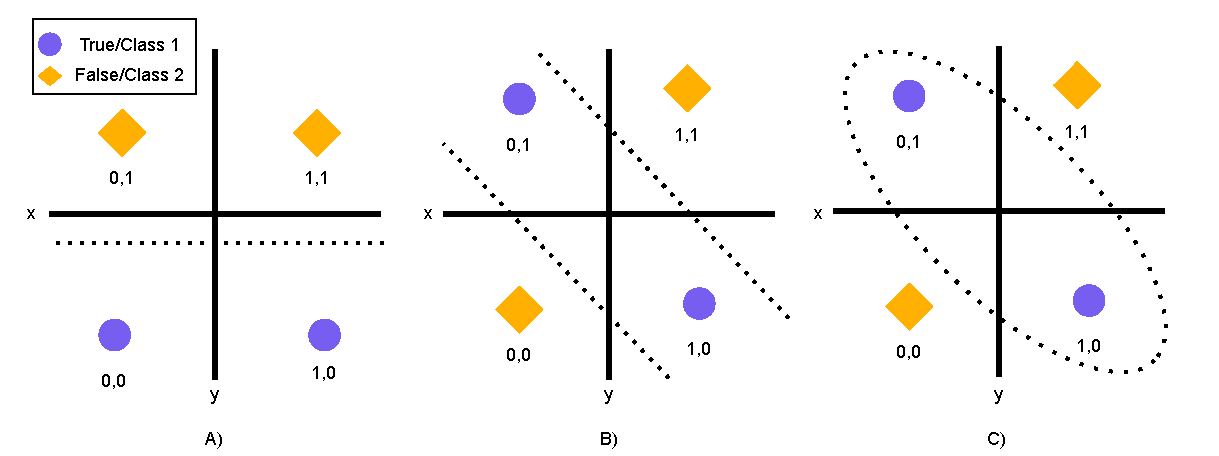
\includegraphics[width=0.6\columnwidth]{../img/xor}
\caption{This picture illustrates XOR problem. Perception can find the correct solution only if the data are linearly separable. It means that they can be divided by a hyperplane. An example of such two-dimensional data can be seen in picture A). The dotted line shows a possible border for separation. Picture B) shows XOR problem. XOR is a logical operation on two boolean variables, which returns true if one variable is True (1) and the other one is False (0), and returns False otherwise. Such data cannot be separated by one hyperplane. Linearly non-separable data can be, for example, separated by a circle (pic. C)}
\label{pic:xor}
\end{figure}

The era of \textit{deep} neural networks started around the year 2007 \citep{Goodfellow-et-al-2016} with bigger datasets and greater computational resources. These two new features opened the possibility of neural network learning without expertly handcrafted parameters tuning with good results.
Many ideas which are currently frequently used are quite old - like backpropagation \citep{Rumelhart} or even the encoder-decoder architecture \citep{Allen19}, \citep{Forcada1997}. However, they became popular only after the development in other computer science areas (mainly because of more advanced hardware) reached a level where they can be trained in a reasonable time.
\par
The basic type of DNN is a multilayer perceptron (see picture \ref{pic:multilayer}).
It is combined with neurons; every neuron has an \textit{activation function}, which is applied to its input. Input to every, but the first layer is a weighted combination of (possibly selection of) neurons from a previous layer. 
Different NN types differ by number and shape of layers, activation functions, and connections between neurons. (see Fig. \ref{pic:multilayer}).
\begin{figure}[ht]
\centering
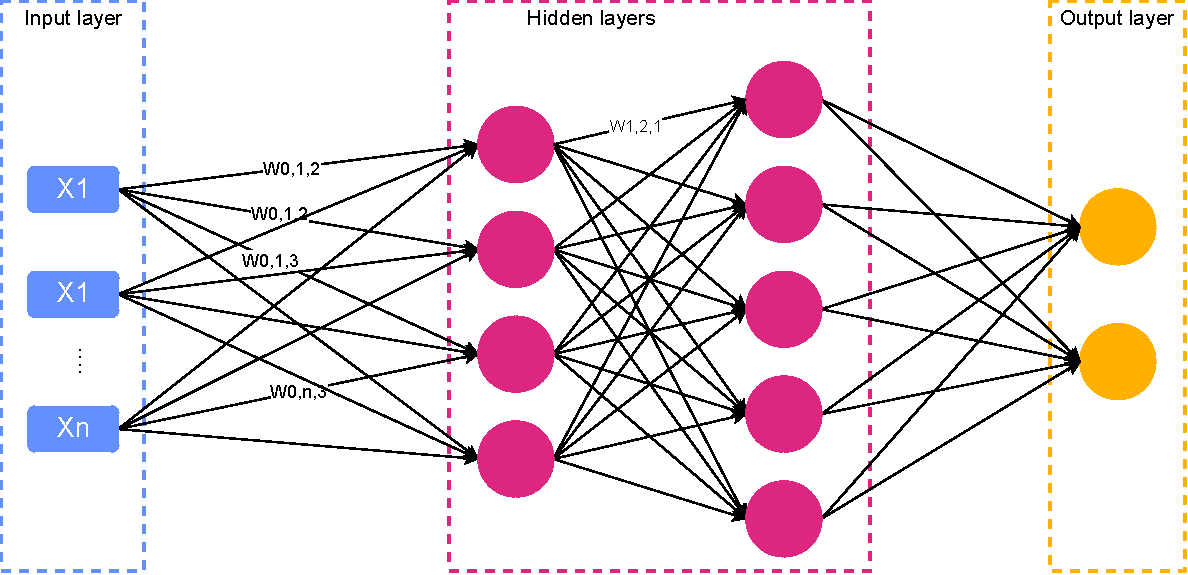
\includegraphics[width=1\columnwidth]{../img/multilayer}
\caption{Multilayer perceptron (or feed-forward neural network) is formed of input and output layer and a variable number of hidden layers with different sizes. In every layer, the chosen application function is applied to a weighted sum of inputs from the previous layer.}
\label{pic:multilayer}
\end{figure}
\par
The following subsections present some of the key ideas for (not only) \acrshort{nlp} and specifically for BERT. In \acrshort{nlp}, the same as in other machine learning methods, it is necessary to decide how to encode the input to make it processable by computers, especially which input features are important for the given task and should be included. These questions are addressed in \acrshort{nlp}, among others, by two techniques: word embeddings (see section \ref{sec:embedd}) and an attention mechanism (see section \ref{sub:attention}). Word embeddings deal with the representation of words and their meaning, while the attention mechanism determines which parts of the text are relevant for a given task. Many machine learning methods are applied to data with no defined order between samples, like images or descriptions of petals for each sample flower\footnote{https://archive.ics.uci.edu/ml/datasets/iris}.
Language data are, however, different because their nature is sequential. Word and sentence ordering is an essential part of the text, and lack of it can make text absolutely sensless. This problem can be more or less satisfactorily handled by Recurrent Neural Networks (section \ref{sub:RNN}) and Transformers architecture (section \ref{sub:transformers}). Combining all these methods led to a BERT models family, which are used in this thesis (see section \ref{sec:bert}).

\subsection{Machine Learning and Regularization}
\label{sub:ml}
Machine learning is a computer science field dealing with algorithms which can learn from experience and improve itself. More precisely, "A computer program is said to learn from experience E with respect to some class of tasks T and performance measure P, if its performance at tasks in T, as measured by P, improves with experience E." \citep{Mitchell1997}. For the techniques examined in this work, experiences are language data -- every single experience is a text. To provide some measure, it is needed to know the ML algorithm's correct output. Many deep learning methods are constructed as \textit{supervised}, which means that every experience has a corresponding label with a correct response (so-called gold data). Metrics used in this case reflect the portion of correctly predicted labels. \citep{Russell1995} Such data structure is handy for the machine learning, but it is hard to obtain them in the required amount because they are usually created manually by humans \footnote{Obviously, if it were already possible to create labels by computers, there would not be necessary to learn it.}. Opposite to this approach are \textit{unsupervised} methods, where no labeled data exists, and metrics are based on different result features (e.g., the compactness of resulting groups). As for tasks, it is possible to distinguish them by the desired outcome between two basic categories: classification and regression. The classification consists of sorting data into one of the predefined classes (e.g., noun, adjective, verb); meanwhile, regression's goal is to predict a numerical result (e.g., expected number of borrowed books in a school library this year).
\par
To be precise, supervised machine learning goal is not to predict all labels correctly in an example data (it would be enough to memorize them), but to predict correctly all possible inputs from the same distribution example data are taken from (find some general features for correct performance). During training, there can appear a problem called \textit{overfitting}. As showed in Figure \ref{pic:overfitting}, overfitting problem is that the result prediction function practically memorized all training data examples and can minimize the error on them very nicely, but probably will not perform well on previously unseen data. A regularization is a tool for preventing such issues. Well known regularization techniques like lasso regression \citep{Tibshirani1996} or ridge regression \citep{Hoerl1970}, which are used for linear regression, work by adding some new members into the sum for the loss function, which should be minimized.
\begin{figure}[ht]
\centering
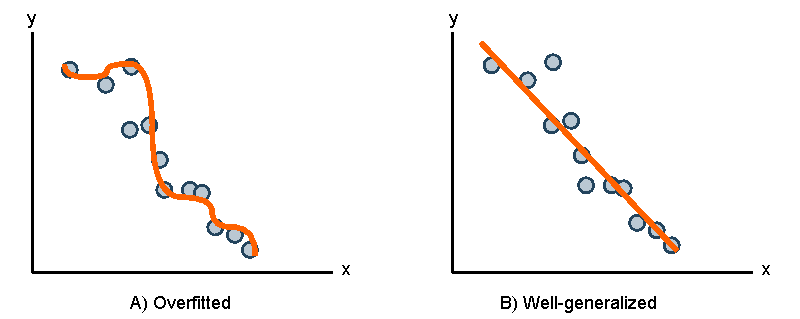
\includegraphics[width=0.7\columnwidth]{../img/overfitting}
\caption{Figure A) presents overfitting scenario. Figure B) illustrates possible well-generalized solution. }
\label{pic:overfitting}
\end{figure}
Another classification regularization method, which is also used in this work, is label smoothing. Label smoothing \citep{Szegedy2015} is an idea applicable to every classification problem, therefore is not limited to an \acrshort{nlp} only.
In any classification task, training data contains labels of the correct classes. In binary classification or one-hot encoded labels, correct class is denoted by 1 and incorrect class(es) by 0 \footnote{One-hot encoding transforms each label into a vector of size K, where n is a number of all possible classes. Than such vector is zero at all position expect the c-th position, where c is the correct class.}. Instead of this, label smoothing applies following formula: 
$$y_{new} = (1 - \epsilon) * y + \epsilon / K,$$ where $K$ is number of classes, $y$ is the original label, $y_{new}$ is the smoothed label and $\epsilon$ is the weight factor. Label smoothing is used as a cure for overfitting and overconfidence in the case of use of a softmax as output activation function. Loss function for softmax classification is: 
 $$ loss = -\sum_{i=1}^{n} \sum_{y=1}^{K} p(y \mid x_i) log \, q_{\theta} ( y_i \mid x_i ) $$
 $p(y \mid x_i)$ being the truth labels' distribution and $q_{\theta} ( y_i \mid x_i )$ being the predicted distribution of labels. After substitution of label smoothing\footnote{\label{note1} Taken from: https://leimao.github.io/blog/Label-Smoothing/}:
$$
loss_{ls} = -\sum_{i=1}^{n} \sum_{y=1}^{K} [(1-\epsilon) p(y \mid x_i)+\epsilon u(y\mid x_i)]log \, q_\theta(y \mid x_i), $$
for $u(y\mid x_i)$ uniform distribution (can be replaced by $1/K$)
which gaves after multiplication \footnote{see footnote \ref{note1}.}:
 \begin{equation} \label{eq:lsloss}
 loss_{ls}= \sum_{i=1}^{n} {(1- \epsilon)[- \sum_{y=1}^{K} p(y\mid x_i) log \, q\theta(y \mid x_i)]+\epsilon [- \sum_{y=1}^{K} u(y \mid x_i)log \, q\theta (y\mid x_i)]}
 \end{equation}
From equation \ref{eq:lsloss} can be seen, then if the network is very confidential about some prediction, the second part of the loss function is very large, so label smoothing works as a regularization of overconfidence.

\subsection{Embeddings}
\label{sec:embedd}
Good performance of \acrshort{nlp} models relies on a text representation. What is hypothetically desired is teaching computers to understand the semantics of the language. Once the computer has a good representation of what given text \textit{means}, it should be easy to answer questions, translate it into another language, etc. Because NN can work only with a numerical representation of inputs, the second requirement upon such language representation is to be numerical. The straightforward way is to represent input words in one-hot encoding. In one-hot representation, a single word is represented by a vector, and one is only at the position of the respective word; all other positions are zeros. Such vector is long as a count of all possible distinct words, therefore it could be quite large. The most important problem of one-hot representation is that each two words are similarly distant from each other. It can be an advantage in some areas, but it is not a correct assumption in linguistics. Words can have similar meanings or be opposite to each other, generally spoken, a distance between them is not uniform.
\par
When compared to one-hot encoding, embeddings  \citep{Bengio2003}, \citep{Ling} are better solution for language data. Embedding is also a vector representing an input word, but in contrast to one-hot encoding, its size does not depend on the vocabulary size. These embeddings are learned by neural networks instead of being prepared by humans. They can be learned for every specific task from scratch, or it is possible to use embeddings trained for usage in many tasks like in the following cases.

\subsubsection{Non-contextualized embeddings}
Before contextualized embeddings appeared, pretrained embeddings were created mainly by Word2Vec \citep{Mikolov2013}, \citep{Turian2010}, \citep{Pennington}, specifically by its two variants: CBOW and SkipGram model.
The objective of CBOW model is to predict a masked word from its context, and SkipGram does precisely the opposite - predicting the context of the given word. These predicting objectives serve just as a tool for forcing a network to learn a useful word representation. Embeddings are then input into a network through a layer with size $number\_of\_words \times embedding\_size$. We still need to bridge the gap between text and numbers, which is possible to do using one-hot encoding or simple word numbering as an input into this first embedding layer.  The problem of Word2Vec-like embeddings is that the embeddings depend only on few nearest words, but the statistics in the dataset are not explicitly used. GloVe \citep{Pennington} embeddings, on the other hand, uses information about frequencies of pairs of words in a whole dataset and are designed to project word vectors into meaningful vector space. 
\\
Embeddings of previously described types use a  context of the word -- it is, in fact, the way how they are meant to work. Similar words are supposed to appear frequently in a similar context. The problem of such embeddings is that an input word embedding in the first layer of the neural network is computed independently on neighbor words, so the same word always has the same embedding regardless of the context. In the case of homonyms, non-contextualized embeddings are a mixture of all the (possibly very different) meanings, which can lead to poor results. %TODO zdroj
The main problem for same word embedding in a different context are homonyms. To solve this problem, contextualized embeddings were developed providing better results universally \citep{Straka2019a}, \citep{Liu2020}.

\subsubsection{Contextualized embeddings}
Contextualized embeddings were invented in recent years, namely BERT \citep{Devlin2019}, ELMo \citep{Peters2018} and XLNet \citep{Yang2019}. %TODO precist \citep{Raffel2019}. 
Their comparison can be found in a subsection \ref{sub:specialBert}. The main difference from non-contextualized embeddings is that same words obtain different meaning according to the sentence they are part of. In addition, they also take into account a larger context than the above-mentioned non-contextual methods. Section \ref{sub:models} describes the possibilities of involving and training such embeddings in more detail.
\par
As embeddings are trained after the input is encoded into one-hot vectors, it is impossible to use pretrained embedding for the encoding of previously unseen words. This problem is solved by embeddings of characters or subwords so that the whole word embedding can be later compound of them. Section \ref{sub:models} describes the possibilities of involving and training such embeddings in more detail. Embeddings are currently the best option of an input representation. \par Another problem is recognizing which parts of the input are valid for the given task. This problem is addressed by the attention mechanism, described in the following subsection. 

\subsection{An Attention mechanism}
\label{sub:attention}
Attention mechanism \citep{Bahdanau} is widely used in \acrshort{nlp} as a tool for extracting relevant information from word sequences. For example, when generating a sentence translation, each word in the target language corresponds to just a few words in the source sentence, not to a whole sentence. Attention gives weights to words, which represents this connections (see picture \ref{pic:att_trans}).

\begin{figure}[ht]
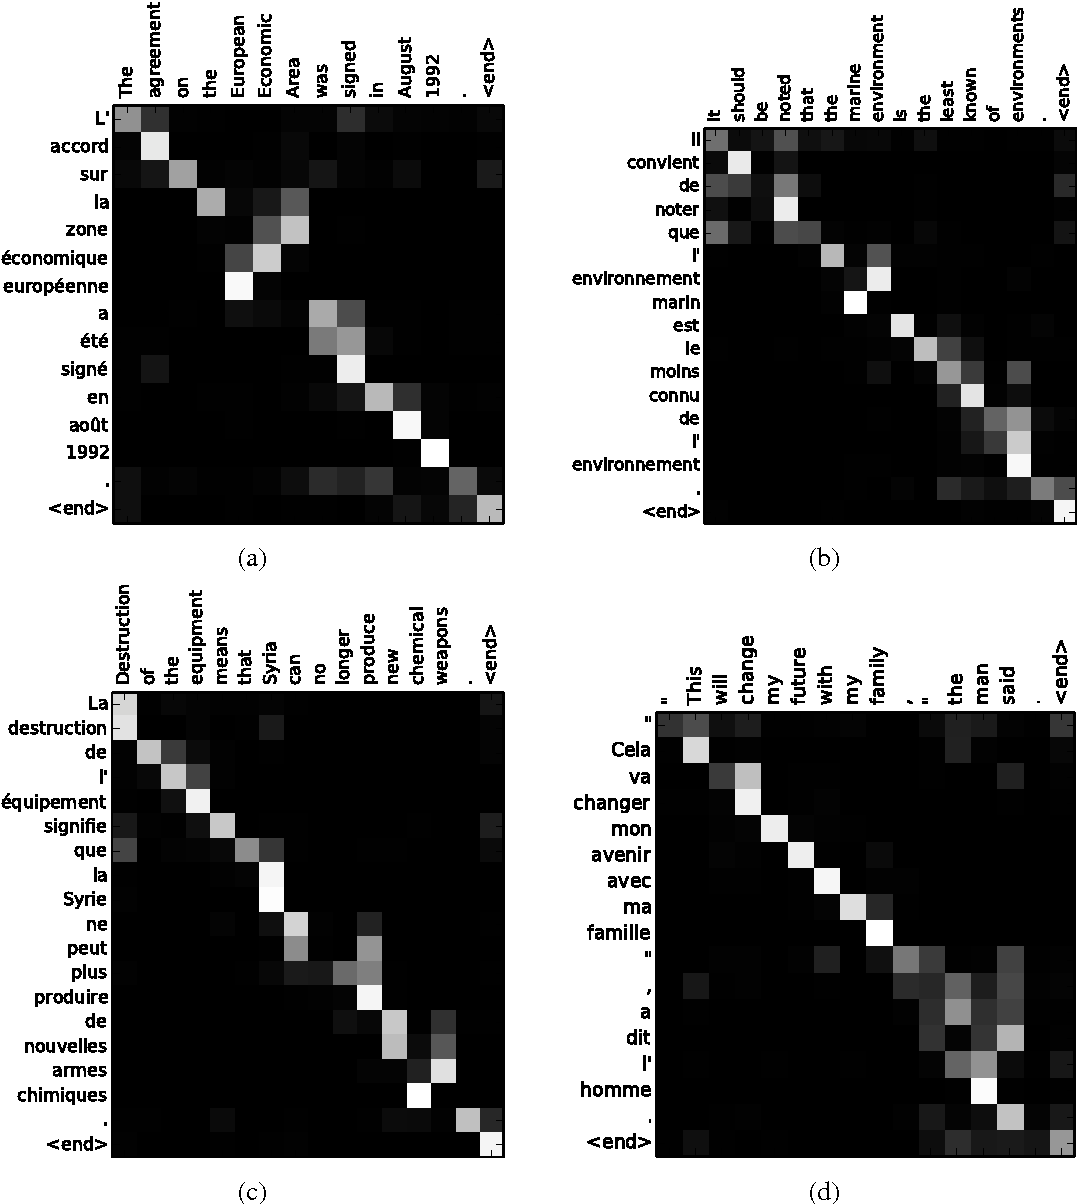
\includegraphics[width=0.7\columnwidth]{../img/attention_translate}
\caption{Figure 3 of \citep{Bahdanau} presents the use of the attention for machine translation. Axis show words of a sentences in English and French. The importance for a translation between a pair of words is represented by a lightness (more lighter = more important).
}
\label{pic:att_trans}
\end{figure}
When the task is a question answering, attention can help a model focus on a relevant part of the text, where the answer is located \citep{Santos2016}.

%\begin{figure}[ht]
%\centering
%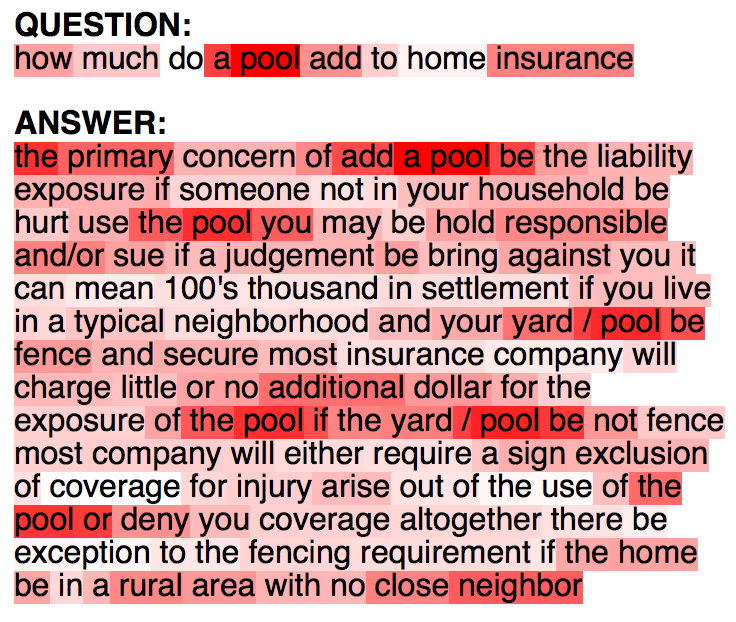
\includegraphics[width=0.7\columnwidth]{../img/attention_cnn}
%\caption{Figure 3 of \citep{Santos2016}
%}
%\label{pic:att_cnn}
%\end{figure}

The same idea can be applied to computer vision, where it imitates human behavior. Humans also focus on (or \textit{attend to}) just a few parts of their visual input when they are, for example, recognizing things in pictures.
Modification to an attention concept, called self-attention \citep{Cheng}, deals with relationships inside one part of the text (e.g., a sentence). This variant of attention does not connect one part of the text (like a question) to another distinct part of the text (like an answer) but only models relationships inside one part. For more explanation, see picture \ref{pic:att_self}
\begin{figure}[ht]
\centering
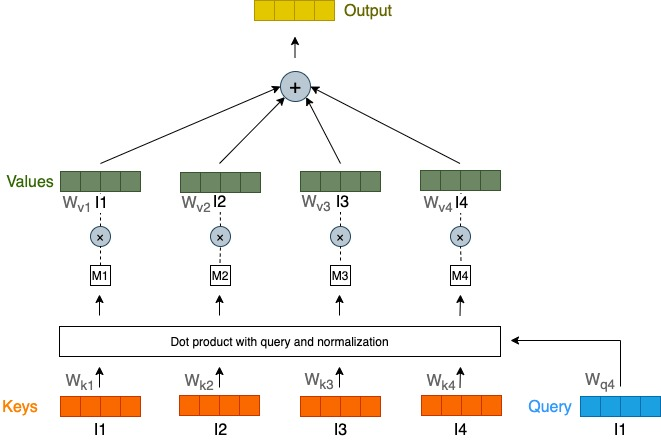
\includegraphics[width=1\columnwidth]{../img/self_attention1}
\caption{Self-attention mechanism scheme for one selected query vector. The result is an embedding, which is improved by the context of the word. This picture illustrates the result for the embedding %TODO jak jako embedding
of the first word (l1) in a four-word long text. Input words are denoted as l1 to l4. Keys , values, and a query are all multiplied by their respective weights ($W_k$, $W_v$, and $W_q$) before any other operation with them. These weights are trained during learning. Dot products between every word and a query are computed. A result is a number for every input word, so four numbers at the end. These numbers are normalized, so the sum of them is equal to 1. These numbers serve as a weight ($M_x$), which indicates the relationship between the query and every other word. The resulting better embedding for the query is then obtained as a sum of the word embeddings weighted by these obtained weights. %zdroj: 10This video series helped me a lot with an understanding of the self-attention concept: https://youtube.com/playlist?list=PL75e0qA87dlG-za8eLI6t0 Pbxafk-cxb
}
\label{pic:att_self}
\end{figure}
An improvement to the self-attention -- \textit{multihead attention} \citep{Vaswani2017} also tries to model relationships between the words in the same sequence. As it is multiheaded, it can, for one word, pay attention to more words (or their parts) (see figure \ref{pic:att_multi}).
\begin{figure}[ht]
\centering
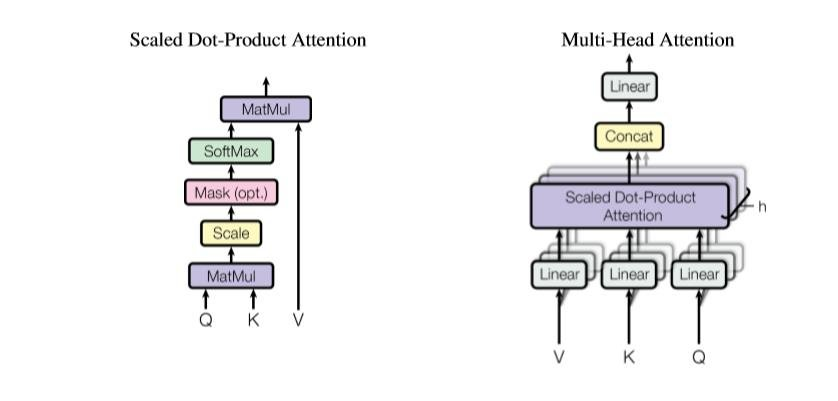
\includegraphics[width=1\columnwidth]{../img/attention_multi}
\caption{Figure 2 from \citep{Vaswani2017} describes the attention mechanism used in Transformers. Scaled Dot-Product Attention, as authors call it, is basically the same architecture as described in the previous figure (\ref{pic:att_self}). The dimension of values ($d_v$) is different from query and keys dimensions ($d_k$). As the normalization serves scaling (division by the number of input dimensions) and than softmax function, which ensures the sum of all weights to be equal to one. Multi-head attention just perform Scaled Dot-Product Attention in parallel and result is then concatenated.
}
\label{pic:att_multi}
\end{figure}
%%%%%%%%%%%%%%%%%%%%%%%%%%%%%%%%%GRU, LSTM, Transformers
\subsection{Recurrent Neural Networks}
\label{sub:RNN}
Text sequences can be very long, and related words often have a long distance in between. This fact places challenging demands on neural networks because such data structure differs from most other NN applications, where input samples are independent, and order does not matter. Text size can also lead to vanishing/exploding gradients because information should be carried for many steps, leading to many multiplications of very small or big numbers in neural networks. %TODO zakže se zapomíná informace
\par
Based on the above mentioned, the construction of neural networks than can capture natural language structure requires solving two issues:
\begin{itemize}
\item input should be understood by the network as a sequence,
\item there must be a possibility to use information from other parts of the sentence (and do not forget them).
\end{itemize}
The first problem was solved by simple Recurrent Neural Networks (RNN). To represent an ordering and a continuity of input words, basic RNN takes the output for previous word as a part of input for the next word (see picture \ref{pic:rnn}). 
 
\begin{figure}[ht]
\centering
\includegraphics[width=1\columnwidth]{../img/rnn}
\protect\caption{Basic Recurrent neural network architecture is showed on the left side of the figure. It is composed by one rnn cell which recurrently uses informations from previously seen input. $X$ is the input of the cell, e.g. a word, $O$ is the output for the given word (e.g. its translation or next word prediction), $V$ is the state passed into another time step. For better illustration of working in the time, RNN can be visualised as a chain of cells connected by a result of previous cell as can be seen on the left side of the figure. Source: \textit{Picture from https://medium.com/deeplearningbrasilia/deep-learning-recurrent-neural-networks-f9482a24d010}.}
\label{pic:rnn}
\end{figure}

The latter problem needs a more complicated approach. There are three attempts to solve this \textit{short memory} of RNN cells -- Gated Recurrent Unit (GRU) \citep{Cho2014}, Long Short Term Memory (LSTM) \citep{Hochreiter1997} and Transformers architecture \citep{Vaswani2017} with an attention mechanism.
\par
Both LSTM and GRU uses an idea of gating. Term \textit{gate} refers to a weight (multiplication factor) for previous informations and new input. Gate determines which information from previous words should be remembered and which should be forgotten. For regulating the memory, the gate is formed by the sigmoid activation function, ranging from 0 to 1 and presenting a portion of remembered information. Previous information is encoded in a cell state and a hidden state %TODO co je cell a hidden state
, both passed from cell to cell (with the application of gates). Comparison of both architectures can be found in figure \ref{pic:lstm_gru}.

\begin{figure}[ht]
\centering
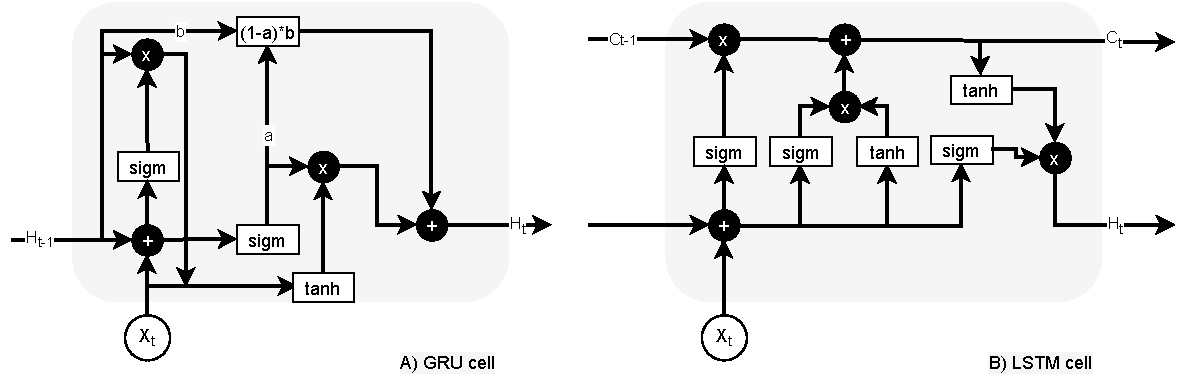
\includegraphics[width=1\columnwidth]{../img/rnn_lstm_gru}
\protect\caption{Comparison of LSTM and GRU architecture. $x_t$ is the current input (current word),  Source: \textit{http://dprogrammer.org/rnn-lstm-gru}.}
\label{pic:lstm_gru}
\end{figure}
\subsubsection*{LSTM} LSTM cell uses three gates: input, output and forget gate. Every gate is composed by a sigmoid function with an actual input and a previous hidden state as inputs.
\textit{Forget gate} filters information from previous cell state. \textit{Input gate} decides which parts of input will affect the results. \textit{Output gate} then selects which part of the result will be actually part of a result. Detailed description can be seen on Figure \ref{pic:lstm_gates}.
\begin{figure}[ht]
\centering
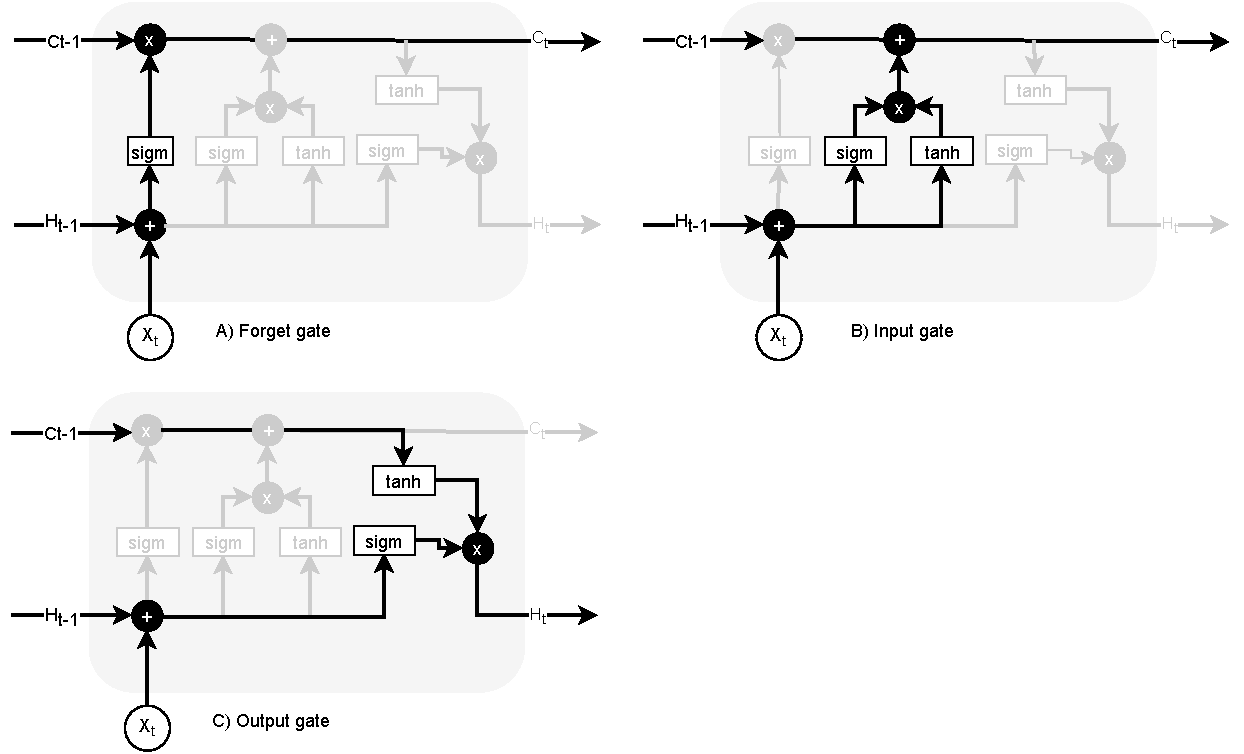
\includegraphics[width=1\columnwidth]{../img/lstm_gates}
\protect\caption{An architecture of the LSTM cell, epsecially its gating mechanism. A LSTM cell carry through the time, in addition to a hidden state, also a cell state, which serves as a long-term memory. \textit{A forget gate} is responsible for choosing the amount of cell state, therefore the information from previous inputs, to be preserved. It uses sigmoid function which returns the output between 0 and 1. \textit{An input gate} controls the addition of new information from the input to the memory. \textit{An output gate} produces the output hidden state which is passed to the next cell. }
\label{pic:lstm_gates}
\end{figure}
%TODO ? Source: \textit{\citep{rnn_paper}}
\subsubsection*{GRU}
GRU also uses gates: reset gate and update gate.
The reset gate is responsible for how much of the previous state will take in the new state. Update gate serves as a weight for a combination of previous and current states, which form the new output. For more detailes see Figure \ref{pic:gru_gates}.
\begin{figure}[ht]
\centering
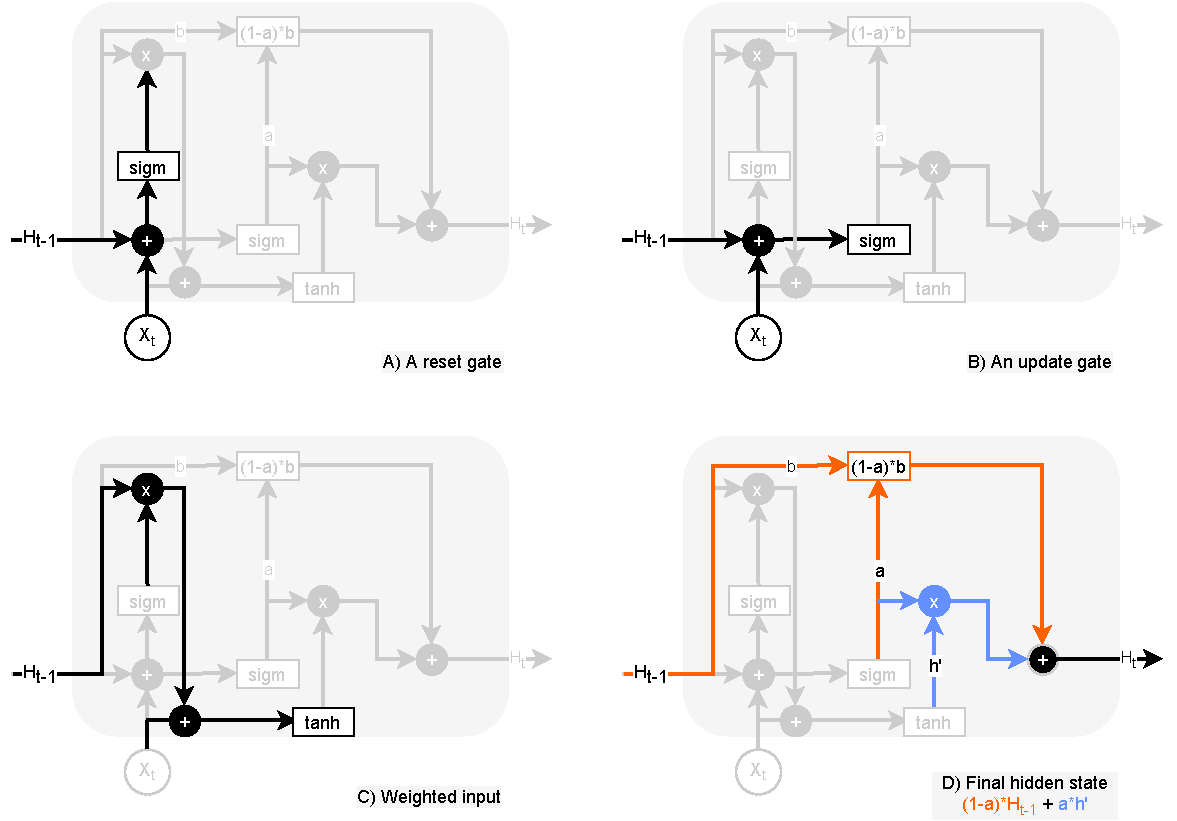
\includegraphics[width=1\columnwidth]{../img/gru_gates}
\protect\caption{An architecture of GRU cell. \textit{An update gate (A)} computes how much of previous information should be passed to next cell based on previous hidden state and the current time input. \textit{A reset gate (B)} uses the same formula (although the input and the previous hidden state have different weights) but serves to a different purpose -- it decides which to forget. \textit{(C)} previous hidden state is weighted by the reset gate before concatenating with current input and normalized via tanh function (to be between $-1$ and $1$) Finally, \textit{new hidden state} is computed as an affine combination of previous hidden state and "normalized" hidden state from previous step.}
\label{pic:gru_gates}
\end{figure}
\subsection{Transformers}
\label{sub:transformers}
The transformers solve the same problem as RNNs but proposes a different architecture. A Tranformers architecture was proposed in 2017, in a paper Attention Is All You Need \citep{Vaswani2017} and essentially depends on a self-attention mechanism (see subsection \ref{sub:attention}). %In the example of sentence processing, attention is able to tell us which other words are important while determining something about the currently processed word. 
Tranformers uses encoder-decoder architecture, which was simultaneously published in 2014 by \citep{Cho2014}, \citep{Sutskever2014} and \citep{Wu2016}. This architecture's basic idea is following: 
This architecture serves to processing of variable-length sequences. Encoder and decoder are connected by a vector of fixed size (context vector), which aims to be a good representation of the input. %TODO pridat obrazek pro porovnani s transformers kde to neni, hlavni zmena v tom paperu
The encoder reads its input and tries to learn such weights that the encoder's final representation of the input contains all important information. This context vector serves as an input into the decoder, which tries to reconstruct the best results. This architecture was first used for machine translation, so the decoder's output, in this case, is a sentence in the target language with the same meaning as an original input (see figures \ref{pic:enco_deco}  and \ref{pic:enco_deco_all}).
\begin{figure}[ht]
\centering
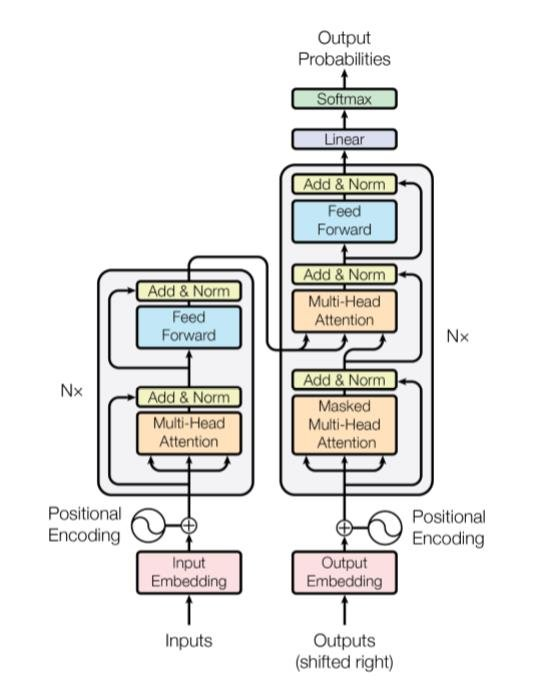
\includegraphics[width=1\columnwidth]{../img/trans_arch}
\protect\caption{This picture describes design of one encoder-decoder block in detail. Every encoder layer consist of self-attention and feed-forward layer supplied with normalization and residual connections. Source: http://jalammar.github.io/illustrated-transformer }
\label{pic:enco_deco}
\end{figure}

\begin{figure}[ht]
\centering
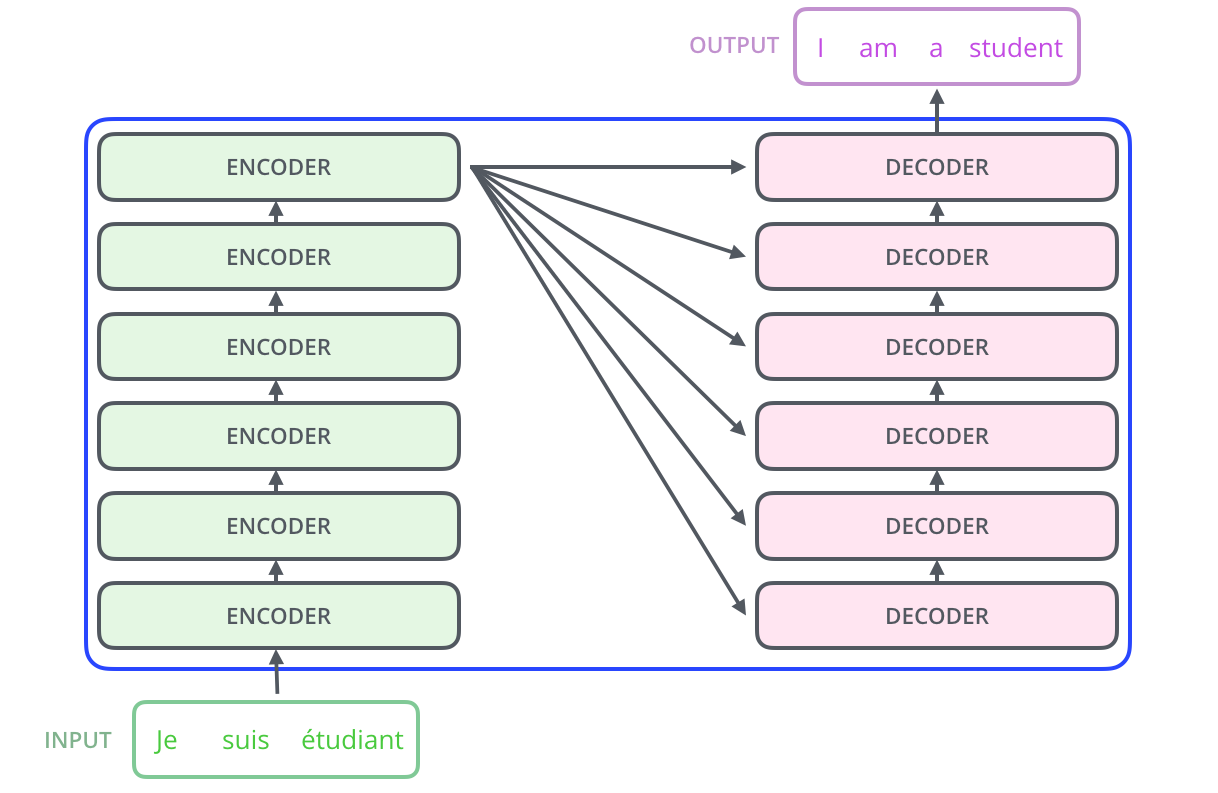
\includegraphics[width=1\columnwidth]{../img/encoder_decoder_all}
\protect\caption{ In transformers, encoder and decoder parts are both composed by many of block of respective types. The input goes first through a series of encoders and than the output of encoder part is put into every decoder in the decoder part. %TODO říct proč
source: http://jalammar.github.io/illustrated-transformer/  }
\label{pic:enco_deco_all}
\end{figure}
A self-attention mechanism is supposed to select the most important words to be focused on and used in many places -- for the input of every encoder layer, for the input of every decoder layer (although masked), and also between encoder and decoder. On the decoder side, the self-attention layer is masked so the decoder can "see" just previous words (there are $-inf$ values in the positions on the right side). For a representation of word position in the sentence (as it is not an RNN cell and it can process all words simultaneously), transformers use position embeddings, which are trained to represent the sentence's ordering.

\subsection{Transfer learning}
\label{sub:models}
Transfer learning is a very important idea because it allows, as the name suggests, to transfer learned knowledge between different tasks. 
%According to bla bla it is leading in industry
Reusing the knowledge can lead to lower training times with fewer demands on technical resources (GPU, CPU) and training data size. It even allows to successfully apply automatic processing into domains where labeled data are not available by transferring the knowledge from another domain with enough training examples. In addition, usage of underlying common knowledge between different tasks can also improve the results of learning algorithms on each task. %Decaf 
One of the first big successes of transfer learning comes from the computer vision field by using models pretrained on ImageNet (currently also on other datasets). ImageNet \citep{Russakovsky2015} is a big dataset of pictures. Every picture is labeled by one of one thousand classes. Many large deep models were trained on this dataset and then applied to different computer vision tasks with a great success \citep{Huh}.  %TODO nekam ze proc to funguje a co vsechno se uci se stale zkouma
\par
Following the taxonomy in figure \ref{pic:tl_taxonomy}, currently most important transfer learning applications in \acrshort{nlp} falls into \textit{sequential transfer learning} category. Machine learning models are first trained on a training objective, and the trained result is then used for a wider set of tasks.
\begin{figure}[ht]
\centering
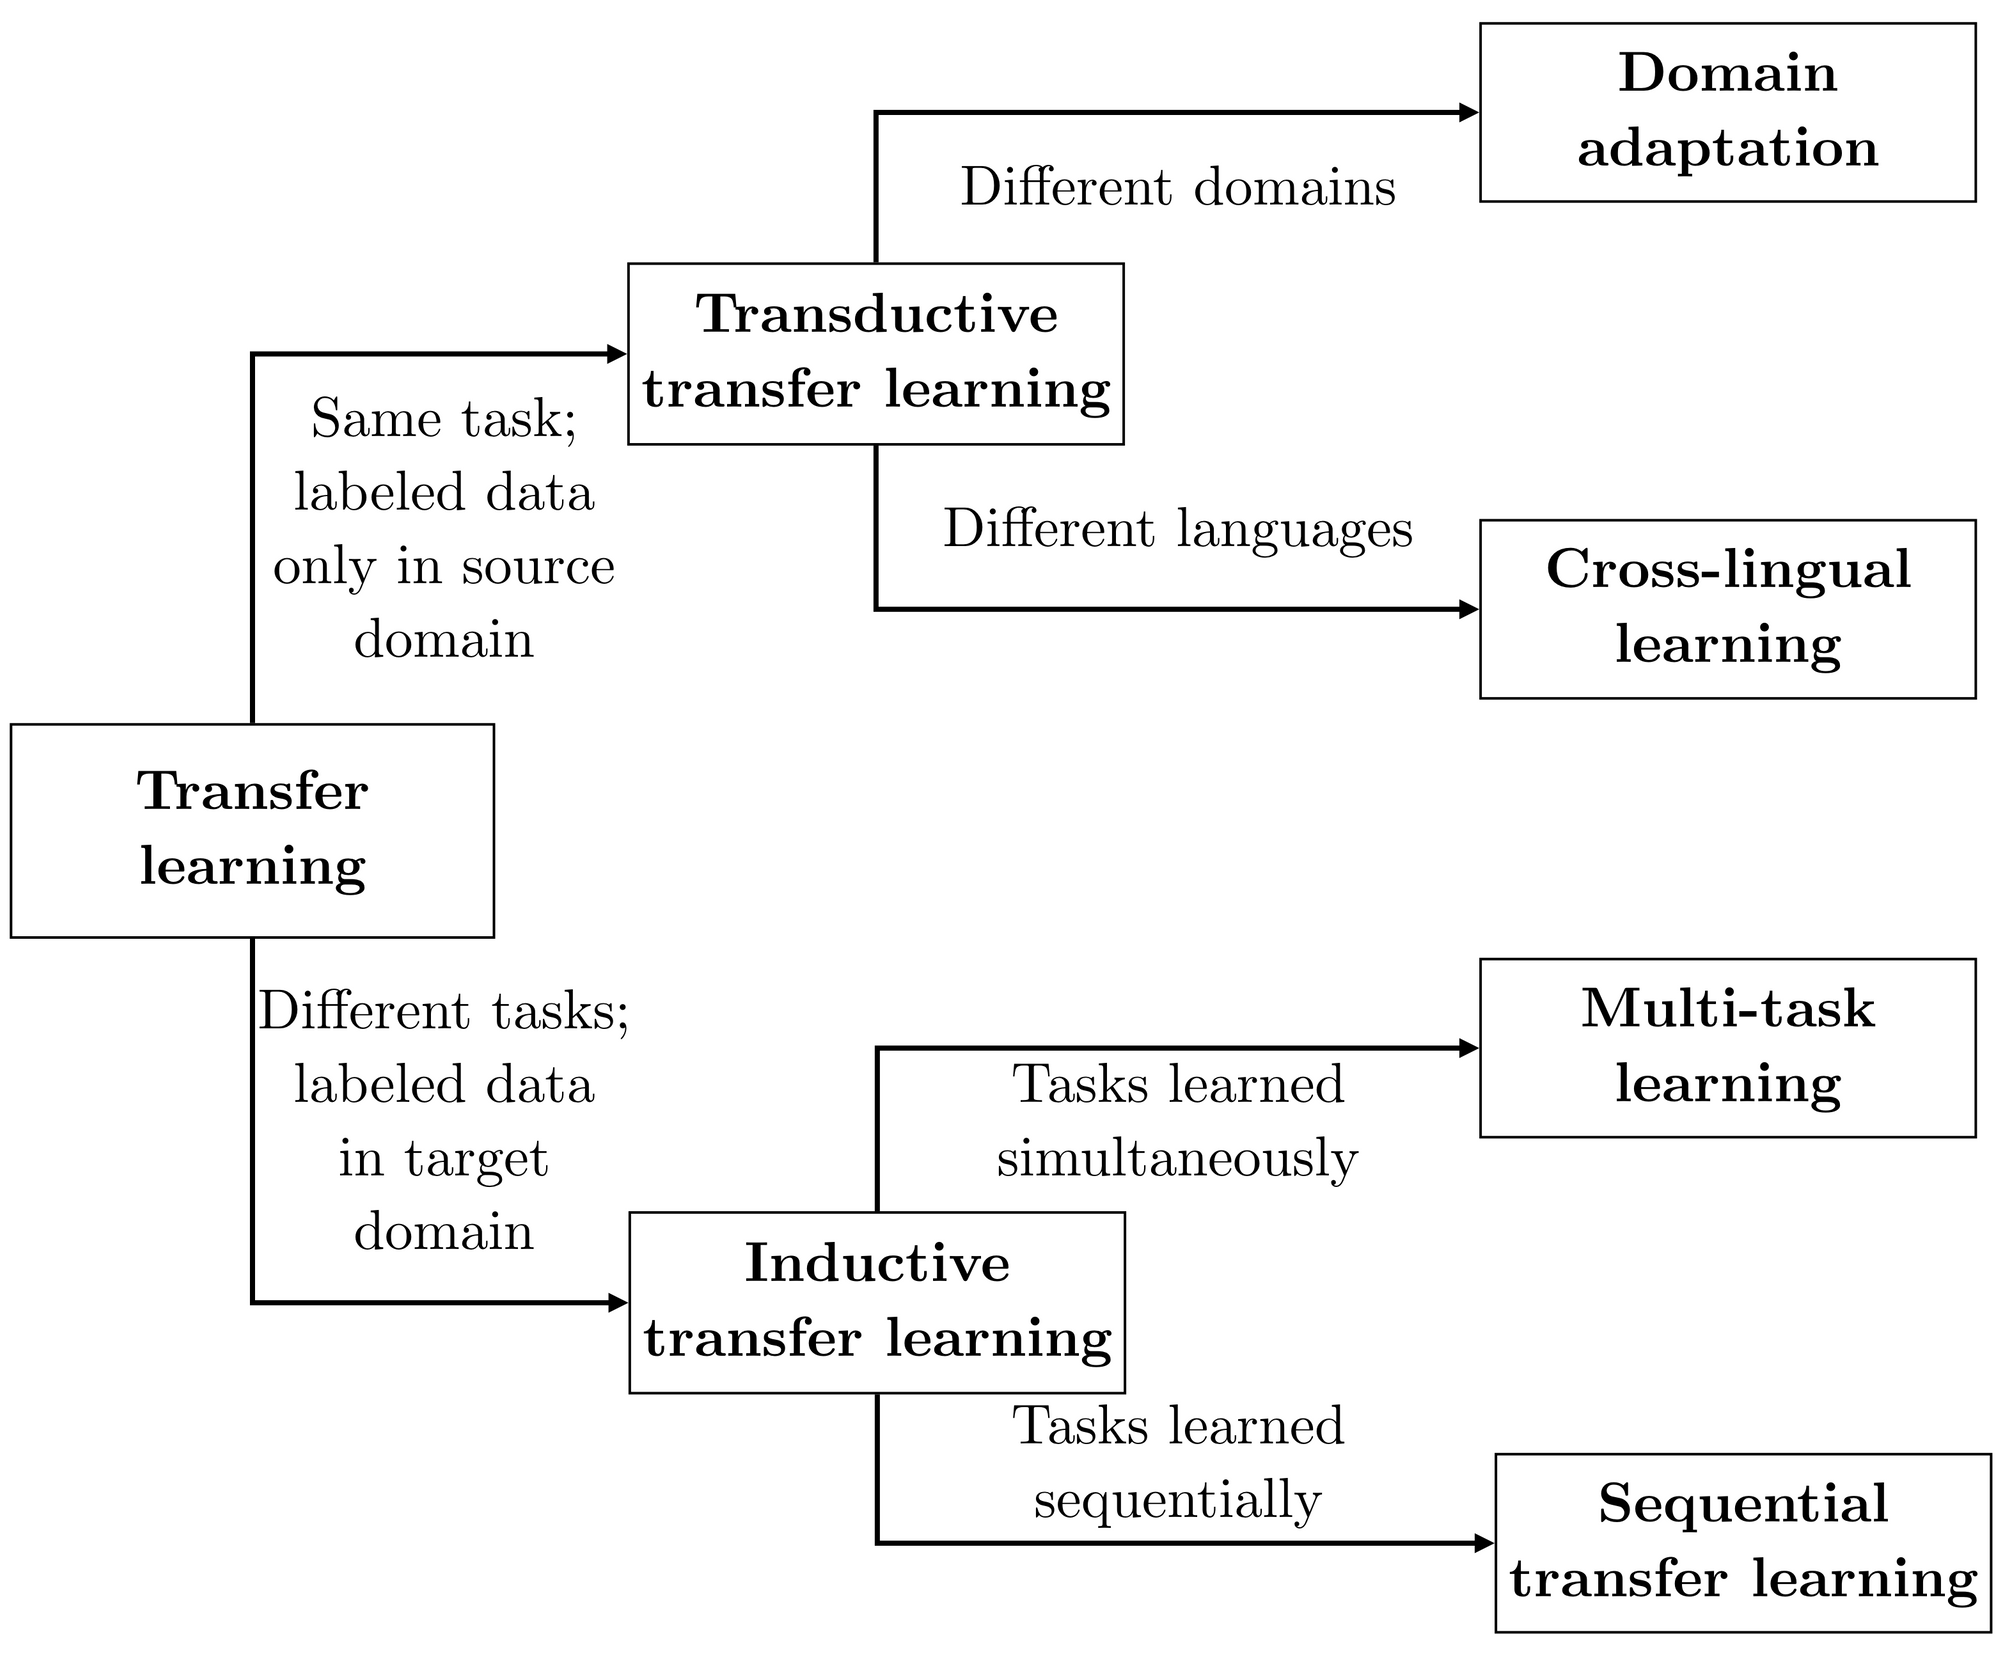
\includegraphics[width=0.7\columnwidth]{../img/tl_taxonomy}
\caption{Figure from \protect\citep{Ruder2019} offers possible taxonomy for transfer learning. %TODO co je to domena, tohle predelat
Following definiton in \citep{Pan2009}, transfer learning's goal is to improve the performance on task $T_1$ from domain $D_1$ by learning knowledge on task $T_0$ from domain $D_0$. Domain is defined as $D = {\chi,P(X)}$, where $X \in \chi$, $\chi$ is a feature space and $P(X)$ is a marginal probability distribution over the feature space. Transfer learning allows the use of trained models on tasks with different sets of labels or different input data's nature. Input data can vary in the source they come from (wikipedia text versus a novel or a social network posts), they can learn from different features (e.g. different languages) or the distribution of classes is different than it was in the training data (so some highly presented classes in training data are rare in this new task and others are quite common but previously not seen too many times).
}
\label{pic:tl_taxonomy}
\end{figure}
For natural language processing, transfer learning is currently mainly represented by contextualized embeddings obtained from pretrained language models.
Contextualization of embeddings is not important only because it solves the problem of homonyms but also because they are believed to store knowledge independent of any language \citep{Feijo2020}, \citep{Hewitt2020}. Contextualized embeddings can be obtained by both supervised or unsupervised learning \citep{Liu2020}. This work focuses on unsupervised learning, as it is currently a promising field according to recent results and because unsupervised learning does not depend on large manually created datasets\footnote{This is a slight terminology inaccuracy. In section \ref{sub:ml}, unsupervised learning was defined as a task where data does not contain correct answer. BERT and derived models, however, use pre-training tasks where the input does not need the manual annotation, but in training itself, individual experiences are provided with the correct answer. Better term introduced by Yann LeCunn \url{https://twitter.com/ylecun/status/1123235709802905600?lang=cs} is \textit{self-supervised}}. Supervised methods use machine translation, which is the classic \acrshort{nlp} task, but also on natural language inference or other tasks with the potential to capture general knowledge about language.
\par
Unsupervised learning tries to learn a language model -- a probability distribution over a sequence of tokens given by the following equation:
 \begin{equation*}
  p(t_1, t_2,...,t_N) =\prod_{i=1}^{N} p(t_i | t_1, t_2, ..., t_{i-1})
\end{equation*}\citep{Liu2020}, where $t_n, N \in \N$ is a sequence of tokens. To reduce this problem, it is possible to consider only fixed size sequences of $n-1$ previous words for every word probability called \textit{n-grams} \citep{Bengio2003}. To achieve the goal of learning a language model, one can use many different tasks, which are believed to force the network to learn useful knowledge about language. First attempts were made with autoencoders (read the text, encode it and try to decode it back) \citep{Dai2015} and machine translation \citep{Ramachandran2017}, but later papers come with better architectures and various new objectives which are described later in section \ref{sec:bert}.  There are generally two ways to transfer learned knowledge \citep{Feijo2020}: extract some representation from the model and use it in another model without changes or modify a model by changing the task-specific layers (so-called head) and \textit{finetune} the whole newly created model for a specific task. There is also a possibility to combine both approaches and, at first, take static features as an input for training, and then when the head starts to perform well, fine-tune the whole model with this better head, so the original weights converge more efficiently to the wanted solution. More detail is offered in \ref{sub:howto}.
%%%%%%%%%%%%%%%%%%%%%%%%%%%%%%%%%%%%%%%%%%%Relevant methods
\section{BERT and its descendants}
\label{sec:bert}
Methods described in previous section
are utilized in the BERT-like models, that belong into a family of contextualized embeddings together with e.g., Contextualize Word Vectors (CoVe) \citep{McCann2017}, \citep{Peters2017}, ELMo \citep{Peters2018}, Flair \citep{Akbik2018}, and series of Generative Pretrained Transformers (GPT) models \citep{Radfort2018}, \citep{RadfordAlec2019}, \citep{Brown2020}. These models are important steps in \acrshort{nlp} progression, which led to BERT family of models. BERT, representing a very effective contextual %TODO contextual contextualized
 embeddings, showed better ability to capture the language knowledge and meant a turning point in the \acrshort{nlp}.
\paragraph{First attempts} to contextual embeddings appeared with two models: the first (CoVe \citep{McCann2017}) uses supervised machine translation and the second (\citep{Peters2017}) uses unsupervised language modeling. Both these models are used for extracting embeddings. These embeddings are concatenated to the non-contextual embeddings (i.e., GloVe) for the target \acrshort{nlp} tasks. CoVe uses a machine translation task (it needs a parallel bilingual dataset) and biLSTM encoder-decoder architecture.  biLSTM are LSTMs, which  process text in both directions.
%which are described in more detail in Figure  %TODO  obrázek.
CoVe, therefore, uses supervised learning, in contrast to the following presented models, which took the path of unsupervised learning as learning from the raw text has a considerable potential due to easy access to a large amount of unlabelled text data (in opposite to labeled datasets, where is almost always not enough data).
\citep{Peters2017} uses an unsupervised method -- language modeling and a concatenation of forward and backward RNN (similarly to CoVe, but uses both GRU and LSTM depending on the task). Both models use last layer as an embedding representation. 
\paragraph{ELMo} is third in the series of biLSTM architecture models and builds on \citep{Peters2017}, but it uses a deeper representation of words. Embeddings are created from a weighted combination of all network layers (in the original ELMo only two layers). This deeper combination was led by the assumption that different network layers are capturing different (but valuable) knowledge. Experiments with weights showed that lower layers tend to capture syntactic information and therefore are more important for syntactic task, while higher layers are important for semantic tasks. 
\paragraph{Flair} also uses unsupervised LM, but the smallest unit of an input is a character, not a word. Flair models the n-th character's probability given the previous characters in the probabilistic description of language modeling. An output is again a word embedding, but this time combined from a representation of its characters. The authors chose this approach to eliminate problems with unknown words.
\paragraph{GPT} by OpenAI (actually in version 3) also uses language modeling for pre-training, but the difference is this time in the architecture. Instead of the LSTM-based RNN network, GPT variants use the decoder part of the transformer architecture and the attention mechanism. GPT also presented deeper architecture than all previously presented methods. GPT 2 version proposes 4 model sizes, with the smallest one having 12 layers and the deepest one with 48 layers. Each layer is a transformer decoder with the self-attention as described in section \ref{sub:attention}. GTP is deeper than ELMo and others but only considers a left context of the word, as the text is processed sequentially in only one direction.
%TODO vsechny obrazek

\subsection{BERT}
On top of all previously mentioned contextual embedding models stands \acrfull{bert} \citep{Devlin2019} with the depth comparable to GPT 2, but using a different part of transformers. It uses modified pre-training tasks compared to other classical language modeling and has a context from both sides. BERT is a pre-trained language model that is finetuned for many other tasks, so it is an example of the transfer learning (see \ref{sub:models}).
To train a language model, original BERT is trained on two tasks -- next sentence prediction and masked language modeling. BERT is proceeding both sides context simultaneously, and due to architecture, in \textit{every layer} every transformer block potentially has information from every other block (and thus from every other word). That is why BERT is called \textbf{deeply} bidirectional or non-directional (because there is no right-to-left or left-to-right direction of processing). BERT is very successful in solving \acrshort{nlp} tasks, although it was surpassed in many tasks by later derived models. 
%TODO tabulky ci graf se zlepsenim za pouziti berta - poslední sota bez berta, první bert a aktuální sota
%TODO nejake vysledky jsou zminene v Erniem
The second part of its popularity is the transfer learning feature of BERT. Resulting BERT model can be used for almost every \acrshort{nlp} task just by changing the classification head. The authors published pre-trained models for English and later also for Chinese and multilingual model and other monolingual models were also published by other authors \footnote{Some published models, which can be used in popular python library Tranformers from HugginFace\footnote{https://huggingface.co/}, can be found here: \url{https://huggingface.co/models}}. Training of the language model requires a considerable amount of data and computational time, but it is needed to be done just once. When the model is trained, it can be used for many tasks by changing the classification head and training only newly added layers or training all layers (but only for a few episodes and with smaller data) and still performing on state-of-the-art level. 
\par
The core of BERT algorithm is based on these three features
\begin{itemize}
\item two unsupervised objectives for pre-training,
\item input embeddings,
\item encoder part of Transformers architecture,
\end{itemize}
and all of them will be described in the following sections.
\subsubsection{Input embeddings}
BERT uses the concatenation of three types of embeddings as an input representation -- token embeddings, position embeddings, and segment embeddings.
\begin{figure}[ht]
\centering
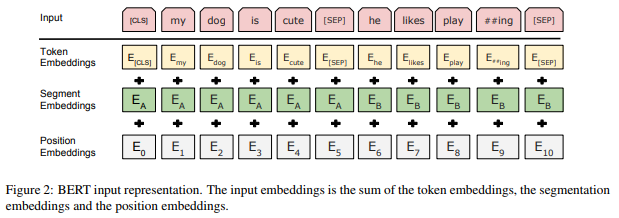
\includegraphics[width=1\columnwidth]{../img/bert_embeddings}
\protect\caption{ An input is represented using three kinds of embeddings for every input word. Every sequence is also marked off by beginning and ending markers (CLS and SEP token), which are also encoded using a combination of all three embedding stypes.
Source: \textit{\citep{Devlin2019}}.}
\label{pic:bert_emb}
\end{figure}
\paragraph{Token embeddings}
The BERT model input can be one or two sequences (not necessarily two sentences, but, e.g., also paragraphs) \footnote{Different terminology is used here than in the original paper. In \citep{Devlin2019}, \textit{sentence} is a term for a whole part of input (fist or second), while a term \textit{sequence} is used for whole BERT input compound of one or two \textit{sentences}.}. All words are split into tokens and converted into embeddings with the use of a pre-trained embeddings model. One word can be tokenized into more tokens because BERT uses WordPiece
embeddings \citep{Wu2016}. WordPiece pre-trained embedding algorithm was originally created for the task of Google voice search for Asian languages and is designed to minimize unknown word tokens. WordPiece model was not pre-trained as a part of BERT paper experiments but represented a quite interesting solution, so that the idea will be briefly explained here.
\par
It is impossible to prepare embeddings for every possible word in a language because this would cause an intractably long embedding size. %TODO proc vlastne u tech co nejsou one-hot? %TODO nekde u layer pouzit shape
Every word which is not a part of the selected embedding set is encoded in the same way (as an unknown word). This situation is not desired because we lost information about words. WordPiece deals with this problem in the following manner: In the first iteration of training, the model creates embeddings only for characters. In every other iteration, some existing model words are concatenated together in a way that causes the highest likelihood of input text. As a result of this method, some words will be embedded as one word, and some will be split into more tokens, as can be seen in figure \ref{pic:bert_inp}.

\begin{figure}[ht]
\centering
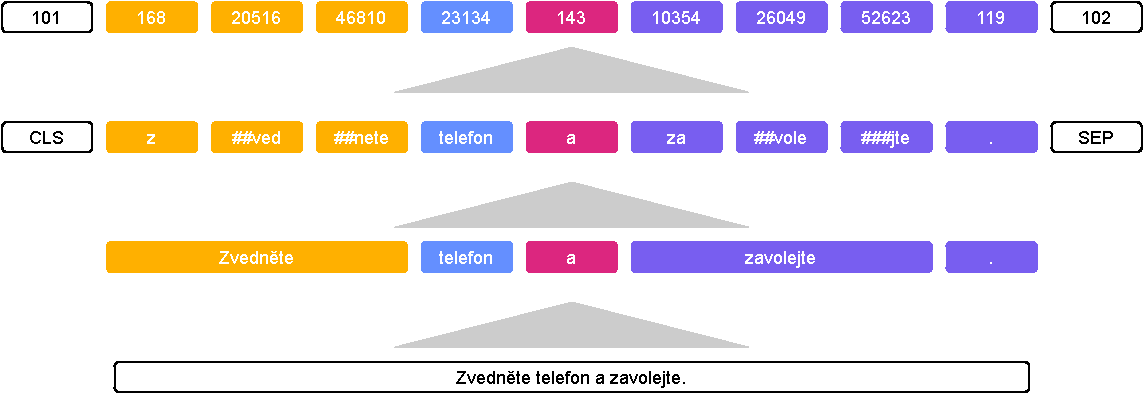
\includegraphics[width=1\columnwidth]{../img/bert_input}
\protect\caption{This figure illustrates a transformation of one input sentence (from PDT3) to suit bert input expectations. The sentence is divided into words and then into tokens from wordpiece tokenizer vocabulary. Accents may be removed depending on the used model. The sentence is decorated with special CLS and SEP tokens to mark the beginning and the end of the sentence. All tokens are then converted into numbers. }
\label{pic:bert_inp}
\end{figure}
\par
Three other tokens are added after this step -- CLS and SEP. 
CLS token is added at the beginning of the input and is used as the first sequence embedding for classification tasks (as sentence analysis). SEP token separates both sequences and is also appended at the end. Whole input transformation can be seen on figure \ref{pic:bert_emb}.
\paragraph{Position embeddings}
All input tokens are processed simultaneously. That is the reason why BERT is often called \textit{undirectional} rather than \textit{bidirectional}. This feature causes an absence of information about the order of tokens. However, the nature of the language is sequential. A bunch of words without an order has no language meaning, and capturing this problem led to recurrent neural networks at first. In BERT is no recurrent cell, and instead, position embeddings solve this problem. They have the same shape as token embeddings (and as segment embeddings), and they are learned the same way as other embedding layers. The original BERT's maximum input size is 512, so this embedding layer should represent positions from 1 to 512. This learning is different from original transformers, where the position was also encoded as embeddings, but embeddings were fixed, not learned.
\paragraph{Segment embeddings}
These embeddings indicate whether the token belongs to the first or second part of the input. They have the same shape as position and token embeddings, and they are also learned. Because BERT input can consist of at most two parts, segment embeddings encode whether the token belongs to the first or second part.
\subsubsection{Architecture}
BERT adapts encoder part of architecture from original Transformers paper   \citep{Vaswani2017} (see section \ref{sub:transformers}).
BERT uses its encoder architecture for each layer, so L encoder layers are finished with one fully connected layer for a specific task (see Fig. \ref{pic:bert_arch}).

\begin{figure}[ht]
\centering
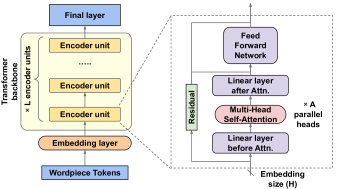
\includegraphics[width=0.8\columnwidth]{../img/bert_arch}
\caption{A figure from \citep{Ganesh2020} describes BERT architecture in detail.}
\label{pic:bert_arch}
\end{figure}

 Original paper proposes two main architecture hyperparameters version, base and large (see table \ref{Tab:base_large}), in the dependence on the number of layers (L), size of the hidden layer (H), and several heads in multi-head self-attention (A). Output before the classification head is a vector of size H for each of the input words. 

\begin{table}
\centering
\begin{tabular}{ |c|c|c| } 
 \hline
    & BERT Base &BERT Large \\ 
 \hline \hline
 L & 12 & 24 \\ \hline
 H & 768 & 1024 \\ \hline
  A & 12 & 16\\ \hline
Total Parameters & 110M & 340M \\\hline
\end{tabular}
\caption{Difference between base and large version of BERT model, as published in 
\citep{Devlin2019}.
} 
\label{Tab:base_large}
\end{table}

\subsubsection{Pre-training tasks}
BERT is pretrained on two unsupervised tasks -- Next Sentence Prediction (NSP) and Masked language modeling (MLM). These two tasks were chosen because BERT's authors believe they can force language models to learn general and valuable knowledge about language.
\paragraph{Next Sentence Prediction}
The input of the BERT model for this task is two sentences, A and B. In 50\% of cases, sentence B is the sentence that follows sentence A in the source text. Otherwise, it is a random sentence from the text. A goal of the task is whether sentence B is following or random, i.e., binary classification. The motivation for this task is a need to represent relationships between sentences, not only between words. Experiments in \citep{
Devlin2019} showed its usefulness for text tasks as question answering. Sentence-level classification with BERT, as in the case of NSP, can be performed by using the last hidden representation of CLS token (the first token of every input example) as an input into classification layer. Authors assumed that this token could work as a summary of the whole sentence, although later work has shown better approaches (i.e., \citep{Liu2019}). 
\paragraph{Masked Language Modeling}
Masked Language Modeling or in other words Cloze task \citep{Taylor1953}
consist of prediction of some missing words in the text. In BERT's case, its implementation follows: 15\% of tokens in each sequence are chosen. For each of these chosen tokens, there is 80\% chance to be replaced by a MASK token, 10\% chance to be replaced by a random token, or it will remain unchanged with 10\% probability. This masking method ensures that the model will try to predict tokens not only in MASK token presence. For backpropagation, only predictions of the MASK token are taken into account. Prediction is made by a softmax function %TODO u kazdeho z 15 procent nebo kde to predpovida?
 whose input is the last hidden representation of the respective token, and the softmax layer outputs a probability distribution for predicting every possible word. 

\subsection{Derived models}
After BERT, many other models built on similar architecture appeared. They all aim to improve the original BERT model in (at least) one of these three methods:
\begin{itemize}
\item A higher efficiency -- original BERT models were trained for about four days on 4/16 TPU for base and large version respectively and are quite memory intensive. Many methods for shortening the training time, memory consumption, or inference time while preserving results were successfully implemented - some of them even outperformed SOTA results stated by BERT.
\item An extension of applicability -- BERT model works nice for tasks requiring sentence or token classification, but is unable of language generation. The original model also does not offer a possibility of connecting knowledge out of the processed text. Both of these problems were explored with well-performing adjusted model architectures as a result \citep{Zhang2019}.
\item Results improvements -- Larger models, longer training times, more data,  better pre-training objectives, and evolved architecture can lead to a significant improvement. Some models only demonstrate scalability with more data, while others win over BERT with more creative pre-training tasks or with a combination of many changes. There is another reason behind these models. It is not completely clear why BERT should work so well, so many authors offer a deep study of individual BERT components' impact on the performance, theoretical explanations, and possible improvements \citep{Yang2019a}, \citep{Liu2019}.
\end{itemize}
 The most famous and important BERT's derivates will be presented in more detail in the following paragraphs.
\paragraph{XLNet} \citep{Yang2019a} solves two theoretical BERT's problems:
\begin{itemize}
\item MASK token, used in BERT's MLM objective, never occurs in real texts. Therefore training data are substantially different from desired practical use, and
\item BERT uses an assumption of independence between MASK tokens, given the unmask words, which does not hold. There definitely could be a strong relationship between two masked tokens in the sequence, even if they are not near each other. Moreover, it is desired for the model to learn such relationships.
\end{itemize}
XLNet presents three basic differences from BERT: presents new training objective (permutation language modeling), uses Transforemers-XL \citep{Dai2019} architecture instead of original Transformers encoders and uses two-stream self-attention. The latter is a consequence of the used objective, which will be briefly explained now. XLNet uses permutations of input sequence's tokens to model each token's probability given the rest of the sequence (bidirectionally). To put it simple, a few of every possible permutation are selected, and then the model learns the probability of the word depending on the previous words in the permuted sentence. As any words are masked, we need to hide the content (=segment and token embeddings) of the chosen token from the network and keep position information. Two-stream self-attention processes these two kinds of information separately, so it is possible to mask out content information. XLNet presents new state-of-the-art results over previous BERT achievements -- with the best models (trained on more data than BERT and four times more training time) and comparable settings (both model and training data sizes).
\paragraph{ERNIE} (= Enhanced Language Representation with Informative Entities)\\ \citep{Zhang2019} enriches BERT with knowledge graphs. This contains knowledge presentation and a selection of objective, which will be able to work with knowledge as well as language information. As for encoding, ERNIE finds all named entities, links them into the knowledge graph, encodes knowledge graph using knowledge embeddings, which forms the input into ERNIE. BERT architecture with transformer encoders is supplemented with knowledge encoders (K-encoders) stacked on the top of text encoders (T-encoders), and the output of the whole model are embeddings for words and entities. The pre-training objective for language is the same as for BERT (NSP and MLM). The authors also present MLM-like objective for knowledge: masking of entities. This model outperforms BERT on knowledge-based tasks (entity typing and relation classification and achieves results comparable to BERT on other \acrshort{nlp} tasks.
 %pridat obrázek 2 
%114M total parameters, N = 6,M = 6, 
\paragraph{RoBERTa} (= Robustly optimized BERT approach) \citep{Liu2019} fall into the third category of BERT family. Great achievements are the result of a thorough exploration of choices made for the original BERT model. RoBERTa uses larger models with more training data (145 GB of uncompressed text more than BERT, which has only 16 GB) and longer training time and offers at least a partial explanation of the influence of architecture, training settings, and objectives on BERT's success. The main differences from BERT are:
\begin{itemize}
\item removing NSP objective, which surprisingly increases the performance,
\item FULL-SENTENCES sampling from the dataset: Every input sample contains full sentences sampled sequentially from data till the maximum size (512) is reached.  Samples may cross boundaries of documents,
\item bigger batch size (2K comparing to 256 of BERT)
\item Byte-level tokens encodings instead of WordPiece, with larger vocabulary size
\item dynamic masking: masks are not selected in advance before pre-training but always created before data enters the model.
\end{itemize}
The resulting architecture is better than BERT, even trained on the same amount of data for the same amount of time.
\paragraph{UNiLM} (= Unified Language Model \citep{Dong2019} enables BERT to generate text. Model architecture corresponds to $BERT_{large}$, but it combined bidirectional BERT training with objectives strengthening usage of a left context, which is important for language generation, and the model also uses NSP. The following rule selects training objectives: 1/3 of time, MLM objective (same as BERT) is used, 1/3 of time model uses sequence-to-sequence language modeling (using previous sentence and all words from left context), and unidirectional language modeling (right-to-left and left-to-right) objectives are used with 1/6 probability. Results are comparable to BERT, with no significant improvement, but the model is able to reach new state-of-the-art on several language generation tasks.
% obrazek s maskami
\paragraph{ELECTRA} (= Efficiently Learning an Encoder that Classifies Token Replacements Accurately) \citep{Clark2020}. ELECTRA presents both more efficiency in training time and improvement on pre-training task. The problem of BERT's MLM task as identified by ELECTRA is its waste of training data. As BERT masks 15\% of tokens and only this serves for model training, almost 85\% of training data are unused. To solve this problem, ELECTRA proposes a new training task, which is defined over all input tokens -- selected tokens are replaced by their alternatives (generated by an additional small network), and the goal for each token is to decide whether it is original or replaced token. Therefore, the model has two parts -- generator and discriminator (loosely inspired by Generative Adversial Networks). It significantly decreases training time because data are used more efficiently. Even with shorter training time, ELELCTRA outperforms both XLNet and RoBERTa.
\paragraph{T5} (= "Text-to-Text Transfer Transformer") \citep{Raffel2019a} is another approach to language generating and also another deep study of various parameters' influence. The training objective is similar to BERT; they choose 15\% of tokens and replace them with the mask token. One change is presented -- it showed to be useful to select whole spans of the text of length three and replace them with one mask token rather than randomly select only words. Final architecture implements encoder-decoder pattern with five different model sizes. Only the two largest models achieved results comparable to BERT and, in the case of the largest one, even outperformed previous state-of-the-art. T5 model uses text-to-text input format. Text-to-text format means that every input is in the text form and also every output. This is natural for some tasks like question answering or translation, but here also tasks with another output type are converted into text and the format is unified for all tasks. The unified format allows the same architecture and training for all tasks and also easy multi-task training.  
\paragraph{BART} (= Bidirectional and Auto-Regressive Transformers) \citep{Lewis2019} is an improvement over BERT, which offers generalization upon previous BERT-like models in terms of training objective and architecture. BART presents the good result in both classification and text generation tasks. BART, similarly to T5, implements encoder-decoder architecture, in this case uniting bidirectional encoder (like BERT) with left-to-right decoder (like in GPT). The main benefit of BART architecture is that it allows arbitrary noising of the input text. Encoder first processes the noised input, and then decoder tries to reproduce the original (not damaged) text. Among many studied possible noises, sentence shuffling and text infilling were proven to be the best, although the performance of various pre-training objectives varied for different tasks. The first objective changes the position of sentences. Text infilling replaces a randomly chosen span of text with MASK token. The span's size is chosen from Poison distribution with $\lambda$ equal to 3 (in contrast to T5, where the size was fixed) and can be zero. Size is comparable to BERT (10\% more parameters). It reaches the performance of BERT and RoBERTa  for comparable tasks and presents a new state-of-the-art in language generation tasks.
%figure 1 ukazuje, jak je related s bertem
\paragraph{Compression of BERT} In addition to models mentioned above, there is a wide range of compression efforts.  In the \citep{Ganesh2020}, authors offer an overview of possible compression methods:
\begin{itemize}
\item data quantization: using fewer bits to represent weights
\item various types of pruning: removing less important weights or components (encoder layers, attention heads)
\item knowledge distillation: involves the large model as a teacher and a smaller model (possibly with completely different architecture) as a student. Student model can learn to imitate different settings of the teacher model (i.e., encoder outputs or output logits)
\item architecture compression: sharing some weights across the model or decrease the vocabulary size of embeddings.
\end{itemize}
This study showed a possibility of reducing BERT to the quarter of original size while preserving performance. One of the famous smaller models is ALBERT (=A Lite BERT) \citep{Lan2019}. ALBERT uses two reduction techniques -- reduces the size of the embedding matrix by approximating it with two smaller matrices and parameters sharing across the layers. In addition to this, ALBERT presents a modification to NSP objective: sentence-order prediction (SOP).
\subsection{How to use language models}
 \label{sub:howto}
 For using BERT-like models in new tasks, there are three possible ways \citep{Liu2020}: 
 \begin{itemize}
 \item feature-based: one data pass through BERT to generate embeddings
 \item fine-tuning: add new classification head(s) and train the whole model
 \item adapter methods: adding task-specific layers between BERT layers and train them for target tasks with other BERT layers frozen \citep{Stickland2019}.
 \end{itemize}
In the first case, the model is used only once to generate embeddings for all input data. These embeddings are stored and later fed to any other \acrshort{nlp} model like regular embeddings. Technically this can be achieved by stacking the second model on the top of BERT and freeze (disable training) on BERT layers, but whit would be time and memory more consuming. This method is valid, and the results will more likely be improved by using BERT embeddings over some other types. Even the BERT paper study shows that using a concatenation of the last four layers can achieve comparable performance to finetuned BERT, but this method still seems to lose some potential of language models compared to learning the model on specific task \citep{Sun}.
\par
Speaking about fine-tuning, there are many decision to be made, i.e., how to chose learning rate, whether to train all layers together or freeze some of them, if its needed to use regularization, which layers to choose as an input into task-specific part of model and many others. There is no guaranteed way, and it could also depend on the task type (sentence vs. token classification), but few typical possibilities which usually work well are known, and main choices with possibilities will be offered here.

\subsubsection{Sequence vs. Token Classification}
Tasks, which BERT can naturally solve fall into two categories -- sequence classification and token classification. The majority of papers seem to focus on sequence classification of sentences or larger text parts, e.g., sentiment analysis, natural language inference, question answering, sentence similarity, etc. Token classification tasks classify each input token, i.e., word, word part, or punctuation mark. The type of task influences the resulting architecture and also brings various problems.
\subsubsection{How to get knowledge from BERT?}
Which information from BERT should go to classification layers is the fundamental question when designing a model. From the horizontal point of view, for sequence classification is mostly used CLS token, but using some combination (e.g., concatenation, mean) of all sequence tokens is also possible \citep{Rogers2020}. Token classification uses an analogical approach -- taking the first token of the word or combining all word's tokens, although it seems to have no impact on the result \citep{Kondratyuk2019}, \citep{Kitaev2018}. As for the vertical combinations, the original BERT paper proposes taking the last layer's representation of respective token(s). Often possibility is a combination of the last four layers (the best option in \citep{Sun} was max). Generally spoken, usage of more layers proved to be advantageous, and it is possible to let the choice of layers be learned \citep{Yang2019b}, \citep{Kondratyuk2019}. %TODO ze ruzne vrstvy vi ruzne veci
\subsubsection{Learning dynamics}
For the learning process itself, the first big question is whether to apply more pre-training on data for the task domain or at least in the task data language as it showed to be beneficial \citep{Sun}. More technical details to be decided are following:

\paragraph{Classification Part Architecture} It is possible to add only one simple classification head on the top of the BERT model or maybe employ the more sophisticated network, e.g., some previous SOTA network, with BERT improving its inputs.
\paragraph{Layers Training} Is it better to train the whole model, only some layers, or should it be dependent on the epoch number? Choosing the suitable scheme can improve the model and prevent catastrophic forgetting \citep{Liu2020}. One of the applicable approaches, proposed initially for different models than BERT, is gradual unfreezing \citep{Ruder2018}, \citep{Chronopoulou2019}. As initially proposed, layers are unfrozen one by one during the training, e.g., one layer is added after each epoch. Because the last layers of the model contain the less general information \citep{Ruder2018}, \citep{Yosinski2014}, it is appropriate to start with the last layer(s) and leave the other layers frozen. After some training, when the model is not a random mess and returns quite decent results, deeper model layers are further trained (finetuned) for few episodes and a significantly lower learning rate. This training practice's motivation is the belief that the original language model captured many generally applicable information about the language and is better than random initialization. Because the model is large and supervised data are usually not so big, it is undesirable to train the whole model, as it can take a long time to convergence and randomly mess up with the trained model's knowledge. After the first training phase, however, the classification head knows the right direction, figuratively speaking, and with the small learning rate, the goal is to customize the language model a bit for current tasks. In addition to gradual unfreezing, it is possible to divide the model only into two parts (BERT part and task-specific part) and train them gradually \citep{Kondratyuk2019}. Multi-stage layerwise training \citep{Yang2020}, designed for BERT, proposes training the output layer with only one encoder layer at a time, which leads to 25\% faster training with good performance.
\paragraph{Learning rate} Right learning rate choice can significantly improve the result. Absolute value of the learning rate for fine-tuning BERT usually lies between $3e^{-6}$ and $5e^{-5}$ \citep{Devlin2019}, \citep{Virtanen2019}, \citep{Kittask2020} as the higher learning rate can cause a catastrophic forgetting \citep{Sun}. Together with its size, learning rate distribution over time and layers is important. Assigning lower learning rate to lower model layers corresponds to the same assumption as in the case of freezing the lower layers, i.e., it is desired to preserve the general information learned during pre-training, and it contributes to the good results \citep{Ruder2018}, \citep{Sun}, \citep{Kondratyuk2019}. Learning rate scheduling as slanted triangular learning rate \citep{Ruder2018}, inverse square root decay (used in \citep{Kondratyuk2019}, \citep{Raffel2019} or linear decay (used in \citep{Liu2019}, \citep{Clark2020}) is an essential component of successful training.
\par
Last, there is also possible to select between different optimizer and different batch sizes. Optimizer seems not to be the most significant part of the decision, as most papers typically do not discuss this choice. Although, in \citep{Chronopoulou2019}, authors present the usage of two different optimizers for different layers -- SGD for pre-trained model layers in order to preserve the learned knowledge and Adam \citep{Kingma2015} for the task-specific layer to support the faster learning. BERT proved to be nicely scalable in selecting the batch size, and simply the bigger batch size usually works better \citep{Liu2019}.
\subsection{Why BERT works?}
\label{sub:specialBert}
It is quite common for deep learning architectures that the reason why they work (especially why they work so well compared to other possibilities) is not visible at first sight. The last part of this chapter focuses on some insight into the language models' functionality. When it comes to examining the inner working of BERT and similar models, two questions arise:
\begin{itemize}
\item What the model knows about the language?
\item Where exactly in the model is all possessed knowledge stored?
\end{itemize}

\subsubsection{What BERT knows about language?}
There are several approaches to research the extent of information that BERT has. The experiments with shuffling or deleting some word showed that BERT probably does not rely too much on syntactic information \citep{Ettinger2019}, \citep{Rogers2020}, although it is present there to some extent as it is possible, for example, extract syntactic trees \citep{Rosa2019}. BERT also contains semantic information of various types. Specifically, experiments indicate a presence of entity types, relations, or semantic roles \citep{Tenney2019a}. BERT possibly "knows" something about the real world but is not able to perform complex reasoning above it \citep{Rogers2020}.

\subsubsection{Where is knowledge stored?}
While searching for the information encoding, it is possible to focus on attention heads or activations in layers.
\citep{Tenney2019} shows that different tasks are solved using different layers, specifically syntactic information is captured by lower layers (or middle layers \citep{Rogers2020}), and semantic information is spread over all layers. The inputs of the last BERT layer (usually used for downstream tasks) serve well as word embeddings, which corresponds with finding the clusters of these embeddings according to word meaning \citep{Rogers2020}. The last layers of BERT are also more task-specific, which leads to possible better transferability of middle layers. A for the attention heads, many papers show that original architecture with sixteen-headed multi-head attention is no optimal, and many heads can be removed in pre-trained models without losing the performance \citep{Michel2019}, which leads to a decrease of inference time. Even a reduction to one head only does not lead to a significant decrease in performance. However, a presence of more heads is better justified during pre-training, at least in early epochs, when the pruning of heads can decrease the performance significantly \citep{Michel2019}. Even though some heads can be redundant, other heads seem to capture specific syntactic relations, e.g, "objects of verbs, determiners of nouns, objects of prepositions, and coreferent mentions" according to \citep{Clark2019}. The same author also shows that CLS token representation in the last layer attends to all words in the sequence, which justifies using these outputs for sequence classification. 
\par
Research of BERT's knowledge representation and storage, together with discoveries presented in the BERT-inspired models, agree that the original architecture leaves a lot of room for improvement or reduction and that "BERT language skills are not as impressive as they seem" \citep{Rogers2020}.

%TODO tabulka - jmeno, training objectives, architecture, bidirectional?, kolik dat, kolik dní, kolik parametrů, jake vsechny tasky

%GPT 2 je vetsi nez bert large\textbf{•}
%tohle z T5 jsou sota. (Devlin et al., 2018; Yang et al., 2019; Dong et al., 2019; Liu et al., 2019c; Lan et al., 2019
%tabulka s treninkovymi casi tu: https://www.borealisai.com/en/blog/understanding-xlnet/

%TODO do lingvisticke casti pospat taky typicke benchmarky squad a glue?

%TODO proc bert funguje:  https://arxiv.org/abs/1908.05620

%Turing NLG a megatron, pouzivaji attention (ale je tam limitation na self attention, proc?) a predict next token




